%% The '5p' and 'times' class options of elsarticle are used for Elsevier CRC
\documentclass[5p,times,authoryear]{elsarticle}

%% The `ecrc' package must be called to make the CRC functionality available
%% ecrc_RIAI es el paquete ecrc de Elsevier con modificaciones para la revista RIAI
\usepackage{ecrc_RIAI}
\usepackage[dvipsnames]{xcolor}
\usepackage{parskip}

%% The ecrc package defines commands needed for running heads and logos.
%% For running heads, you can set the journal name, the volume, the starting page and the authors
%%%%%%%%%%%%%%%%%%%%%%%%%%%%%%%%% Aaadido por Secretaraa RIAI

\usepackage[spanish]{babel}

%\usepackage[spanish]{babel}
\usepackage[utf8]{inputenc}% Idioma
\addto\captionsspanish{%
\def\tablename{Tabla}}
\usepackage{amsmath}            % Para las referencias a ecuaciones con \eqref
\usepackage{epstopdf}           % Para poder insertar figuras .eps al compilar con PDFLATEX
\usepackage{flushend}           % Para igualar las columnas de la altima pagina
%\usepackage{hyperref}           % Para hipervanculos dentro del PDF
%%%%%%%%%%%%%%%%%%%%%%%%%%%%%%%%%%%%%%%%%%%%%%%%%%%%%%%

% set the starting page if not 1
\firstpage{1}

%% Give the author list to appear in the running head
%% Example \runauth{C.V. Radhakrishnan et al.}
\runauth{Ayala Franklin et al.}

%% The choice of journal logo is determined by the \jid and \jnltitlelogo commands.
%% A user-supplied logo with the name <\jid>logo.pdf will be inserted if present.
%% e.g. if \jid{yspmi} the system will look for a file yspmilogo.pdf
%% Otherwise the content of \jnltitlelogo will be set between horizontal lines as a default logo

%% Give the abbreviation of the Journal. Contast the Publisher if in doubt what this is.
%\jid{RIAI}

%% Give a short journal name for the dummy logo (if needed)
%\jnltitlelogo{}

%% Hereafter the template follows `elsarticle'.
%% For more details see the existing template files elsarticle-template-harv.tex and elsarticle-template-num.tex.

%% Elsevier CRC generally uses a numbered reference style
%% For this, the conventions of elsarticle-template-num.tex should be followed (included below)
%% If using BibTeX, use the style file elsarticle-num.bst

%% End of ecrc-specific commands
%%%%%%%%%%%%%%%%%%%%%%%%%%%%%%%%%%%%%%%%%%%%%%%%%%%%%%%%%%%%%%%%%%%%%%%%%%

%% The amssymb package provides various useful mathematical symbols
\usepackage{amssymb}
%% The amsthm package provides extended theorem environments
%% \usepackage{amsthm}

%% The lineno packages adds line numbers. Start line numbering with
%% \begin{linenumbers}, end it with \end{linenumbers}. Or switch it on
%% for the whole article with \linenumbers after \end{frontmatter}.
%% \usepackage{lineno}

%% natbib.sty is loaded by default. However, natbib options can be
%% provided with \biboptions{...} command. Following options are
%% valid:

%%   round  -  round parentheses are used (default)
%%   square -  square brackets are used   [option]
%%   curly  -  curly braces are used      {option}
%%   angle  -  angle brackets are used    <option>
%%   semicolon  -  multiple citations separated by semi-colon
%%   colon  - same as semicolon, an earlier confusion
%%   comma  -  separated by comma
%%   numbers-  selects numerical citations
%%   super  -  numerical citations as superscripts
%%   sort   -  sorts multiple citations according to order in ref. list
%%   sort&compress   -  like sort, but also compresses numerical citations
%%   compress - compresses without sorting
%%
%% \biboptions{comma,round}

% \biboptions{}

% if you have landscape tables
\usepackage[figuresright]{rotating}

% put your own definitions here:
%   \newcommand{\cZ}{\cal{Z}}
%   \newtheorem{def}{Definition}[section]
%   ...

% add words to TeX's hyphenation exception list
%\hyphenation{author another created financial paper re-commend-ed Post-Script}

% para poder introducir varias figuras que ocupen el ancho de las dos columnas.
\usepackage{subfigure}

% declarations for front matter


\begin{document}

\begin{frontmatter}

%% Title, authors and addresses

%% use the tnoteref command within \title for footnotes;
%% use the tnotetext command for the associated footnote;

%% use the fnref command within \author or \address for footnotes;
%% use the fntext command for the associated footnote;

%% use the corref command within \author for corresponding author footnotes;
%% use the cortext command for the associated footnote;
%% use the ead command for the email address,
%% and the form \ead[url] for the home page:
%%
%% \title{Title\tnoteref{label1}}
%% \tnotetext[label1]{}
%% \author{Name\corref{cor1}\fnref{label2}}
%% \ead{email address}
%% \ead[url]{home page}
%% \fntext[label2]{}
%% \cortext[cor1]{}
%% \address{Address\fnref{label3}}
%% \fntext[label3]{}

%\dochead{Cabecera artaculo}
%% Use \dochead if there is an article header, e.g. \dochead{Short communication}

\title{Serie de nivel del mar si 2}

%% use optional labels to link authors explicitly to addresses:
%% \author[label1,label2]{<author name>}
%% \address[label1]{<address>}
%% \address[label2]{<address>}

\author[First]{Franklin Farid Ayala Cruz\corref{cor1}\fnref{label2}}
\ead{ffayalac@unal.edu.co}

\author[Second]{Johann K. Delgado}
\ead{jkdelgadog@unal.edu.co}

\author[Third]{Andrés F. Osorio}
\ead{afosorioar@unal.edu.co}

\fntext[label2]{Nota al pie para el autor 1}
\cortext[cor1]{Autor en correspondencia.}

\address[First]{Ingeniería Civil, Universidad Nacional de Colombia, Sede Medellín, Colombia}
\address[Second]{OCEANICOS Research Group, Universidad Nacional de Colombia, Sede Medellín, Colombia}
\address[Third]{OCEANICOS Research Group, Universidad Nacional de Colombia, Sede Medellín, Colombia}


\begin{abstract}
%% Text of abstract

El estudio de las variables hidrodinámicas oceánicas que inciden en la costa provee un conocimiento báscio de las condiciones que alteran la geomorfología de las playas. Variables tales como el nivel del mar, el período pico, la altura de ola significante y la dirección media del oleaje son estuadiadas con el fin de conocer su efecto en un problema de erosión en uno de los lados que da al mar de la Isla Punta Soldado, Buenaventura. Por lo tanto, es necesario realizar un análisis estadístico de los regímenes medios y extremos para propagar el oleaje que genere las condiciones geomorfológicas actuales de la isla.

\end{abstract}

\begin{keyword}
%% keywords here, in the form: keyword \sep keyword

%% MSC codes here, in the form: \MSC code \sep code
%% or \MSC[2008] code \sep code (2000 is the default)

Geomorfología \sep erosión \sep oleaje 

\end{keyword}

\end{frontmatter}

%%
%% Start line numbering here if you want
%%
% \linenumbers

%% main text
\section{Introducción}

La acción de diferentes fenómenos como el viento, perturbaciones meteorológicas, tsunamis y demás (llamados generalmente \textit{forzadores}) ocasionan perturbaciones en las masa de agua oceánicas llamadas olas. Cuando el viento actúa como el principal generador en alguna zona, el oleaje allí es más caótico, desordenado e irregular y se conoce como tipo \textit{sea}. A medida que este oleaje se va propagando, ocurren una serie de fenómenos que lo ordenan en trenes de onda y pierde en buena medida su irregularidad, este oleaje es de tipo \textit{swell}.

Cuando en una zona existe un solo tipo de oleaje, ya sea \textit{sea } o \textit{swell}, basta con determinar los parámetros integrales del oleaje: Altura de ola significante, período pico, período medio y dirección media. Dado que en muchos lugares esta situación no ocurre, sino que convergen 2 o más sistemas de oleaje, las técnicas de análisis se vuelven más complejas y se recurre a análisis espectral, este análisis permite una mayor aproximación a las condiciones que realmente se presentan en estas zonas.

En el pacifico colombiano, las condiciones meteorológicas locales están influenciadas por: a) La zona de convergencia intertropical (ZCIT), la cual se mueve según otros eventos macrolimáticos, a) Los tres chorros (Tehuantepec, Papagayo y Panamá) provenientes de los gradientes de presión entre norteamérica y el caribe-pacífico, c) el cinturón de tormentas extratropicales que genera un oleaje propagado a través de largas distancias que arriva a las playas en forma de \textit{swell}.

Según lo descrito, en el pacífico colombiano interactuán más de dos sistemas de oleaje que no podrían ser analizados de una forma verídica con parámetros integrales del oleaje, por lo tanto, el estudio de este fenómeno debería realizarse a través de las condiciones espectrales que existen.

Dado que las técnicas de descomposición espectral de los tipos de oleaje incidentes no son bien dominadas, se asume que los valores de los parámetros del oleaje (dirección, periodo y altura de ola) están incluyendo los espectros existentes (\textbf{CITAR}). Estos parámetros componen el régimen medio usado para la determinación de las condiciones de frontera de los modelos de propagación de oleaje.

Para estalecer estas condiciones medias, se deben buscar fuentes de datos con registros fiables, en su preferencia continuos y con las menores resoluciones espaciales. Siguiendo esta línea de requisitos, hay tres fuentes de datos disponibles: Datos de boyas, datos satelitáles y datos de reanálisis. Los datos de las boyas están disponibles para 3 años (2008-2010) con frecuencias del orden de días para los años 2008 y 2010 y del orden de horas para el año 2009. Los datos de reanálisis están a una resolución espacial de 0.5x0.5 grados y una resolución temporal horaria. Los datos satelitales tienen frecuencias de medición muy aleatorias y resoluciones espaciales confusas, dado que el satélite aunque realiza tomas puntuales, su órbita lo lleva a realizar un barrido muchas veces no homogéneo.

La zona de estudio se describe a continuación:

\begin{figure}[h]
    \centering
    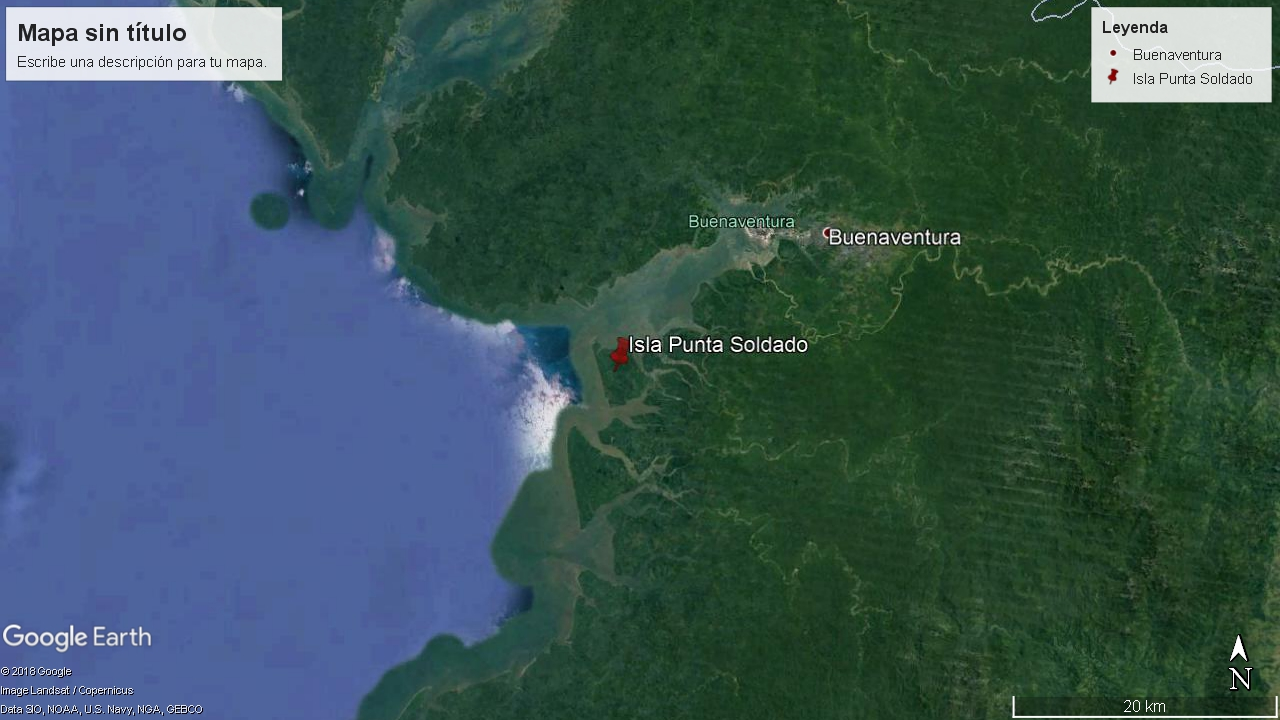
\includegraphics[scale=0.25]{Graficas/Zona}
    \caption{Zona de estudio}
    \label{fig:0}
\end{figure}

Basados en lo descrito anteriormente, se plantea el objetivo de este estudio como la caracterización del regímen medio de oleaje y marea en la Isla Punta Soldado, ubicada en la costa pacífica colombiana, específicamente en la bahía de Buenaventura.

\section{Métodos y fuentes de información}

\subsection{Fuentes de información}

\subsubsection{Datos be boyas}

La boya 32487 es la única estación cercana a la bahía de Buenaventura con registros de parámetros de oleaje disponibles y está adscrita al \textit{National Data Buoy Center (NOAA)}, su ubicación es 3.517N 77.737W. Los años de los registros son 2008, 2009 y 2010 y entre los parámetros existentes están: Período de ola dominante, período de oleaje medio y altura de ola significante. Los registros de 2008 y 2009 presentan una longitud pequeña y discontinua, por lo que es difícil determinar una frecuencia de medición específica. La serie del 2009 posee una cantidad de registros cercana a los 8760 datos, lo que lleva a inferir que la frecuencia de medición estuvo cercana a la horaria. Esta última serie servirá para realizar una comparación con las demás fuentes de datos y evaluar su confiabilidad, dado que es la más continua de las 3 existentes y es la que representa los datos reales de la zona de estudio.


\subsubsection{Datos de satélite}

En la red abierta de datos oceánicos australiana (AODN) existen las series de mediciones de diferentes misiones satelitales, es importante aclarar que estas mediciones son secundarias a los objetivos principales que tienen estos satélites, y por ende su calidad no es la mejor. La forma en la que estos satélites logran obtener series de altura de ola es a través una tecnica llamada altimetría. El principio fundamental de esta técnica es la superposición de imágenes tomadas por un satélite y el análisis de estas para su correlación con la altura de ola. Según sea el tipo de banda (c, Ku, Ka) en el que emite el satélite será el ajuste qué se debe realizar \textbf{CITAR}. Debido a la forma en la que orbita un satelite la superposición de imágenes se da bajo la medición en puntos diferentes, esto agrega incertidumbre a los valores finales, puesto que no se puede asumir un solo lugar de medición. Para fines prácticos se asume el promedio de las longitudes y de las latitudes, como el punto especifico en el que se midió.

Con el objetivo de comparar las series existentes con respecto a la estación 32487 se descargaron los datos más cercanos a este lugar y que estén en el rango de tiempo de comparación, es decir 2009. La única misión con datos para ese año y en una región espacial relativamente cercana es Sentinel 3. Debe recordarse que no existen valores de período medio, período pico y dirección media del oleaje.  

\subsubsection{Datos de reanálisis}

Los datos de reanálasis fueron obtenidos del centro europeo de pronósticos meteorológicos a medio plazo (ECMWF), esta información surge de un proceso compuesto por registros históricos y una técnica llamada asimilación, en este proceso se emplean modelos de propagación de oleaje que ayuden a determinar los valores de los parámetros en tiempos y ubicaciones que no los tienen medidos. El modelo usado para propagación es WWACH 3 \textbf{AMPLIAR}. Es importante hacer la salvedad que este modelo tiene un uso apropiado en zonas de aguas profundas, dado que en zonas de aguas intermedias y sómeras (como lo es regularmente cerca a la plataforma continental) aparece un ruido generado por el lecho marino. Esta condición deberá tenerse en cuenta para el uso posterior de los datos. Dentro de las diferentes variables que existen, se decargan solamente el período pico, la altura de ola significante y la dirección media del oleaje.

\textbf{Revisar condiciones de aguas profundas}

\subsubsection{Datos de mareógrafo}
La comisión oceanográfica intergubernamental de la UNESCO ha reunido un conjunto de estaciones de medición de nivel del mar, dentro de las cuáles está el mareográfo de Buenaventura (Código: \textit{Buve}: 3.8906,-77.0808) operado por la CIOH con registros de nivel del mar desde 1970 a una resolución horaria y diaria. En ambas resoluciones existen vacíos en los registros que pueden ser debidos a mantenimiento del equipo o inclusive reemplazo del mismo, puesto que existen desde el orden de días hasta el orden de meses. Estas series serán empleadas para el análisis de marea en la zona de estudio.

\subsection{Comparación entre fuentes de datos}
Dado que para el oleaje existen tres fuentes de datos diferentes debe determinarse la que se va a emplear para el análisis de régimen medio, por lo tanto, se decidió realizar una comparación entre la serie de 2009 de la boya y las series de reanálisis y satélite existentes en el mismo intervalo de tiempo y en las ubicaciones más próximas a la boya (Tabla \ref{tab:ubic espaciales}); claramente las resoluciones de los satélites y del reanálisis no permiten una ubicación exactamente igual.

\begin{table}[h]
    \centering
    \begin{tabular}{c|c}
         \bf{Fuente} & \bf{Ubicación}\\
         \hline
         Boya & 3.517 N 77.737 W \\
         \hline
         Satélite & Región 0.1x0.1 grados\\
         \hline
         Reanálisis & 3.5 N 272.5 W \\
    \end{tabular}
    \caption{Localizaciones espaciales de las series temporales de altura de ola significante y periodo pico}
    \label{tab:ubic espaciales}
\end{table}

Inicialmente, se presentan las series temporales de $H_s$ descargadas para el año 2009 (Fig. \ref{fig:1}). Puede notarse que la resolución de los satélites es muy pobre respecto a la boya y el reanálisis, esto lleva a que se descarten los datos provenientes de satélite

\begin{figure}[h]
    \centering
    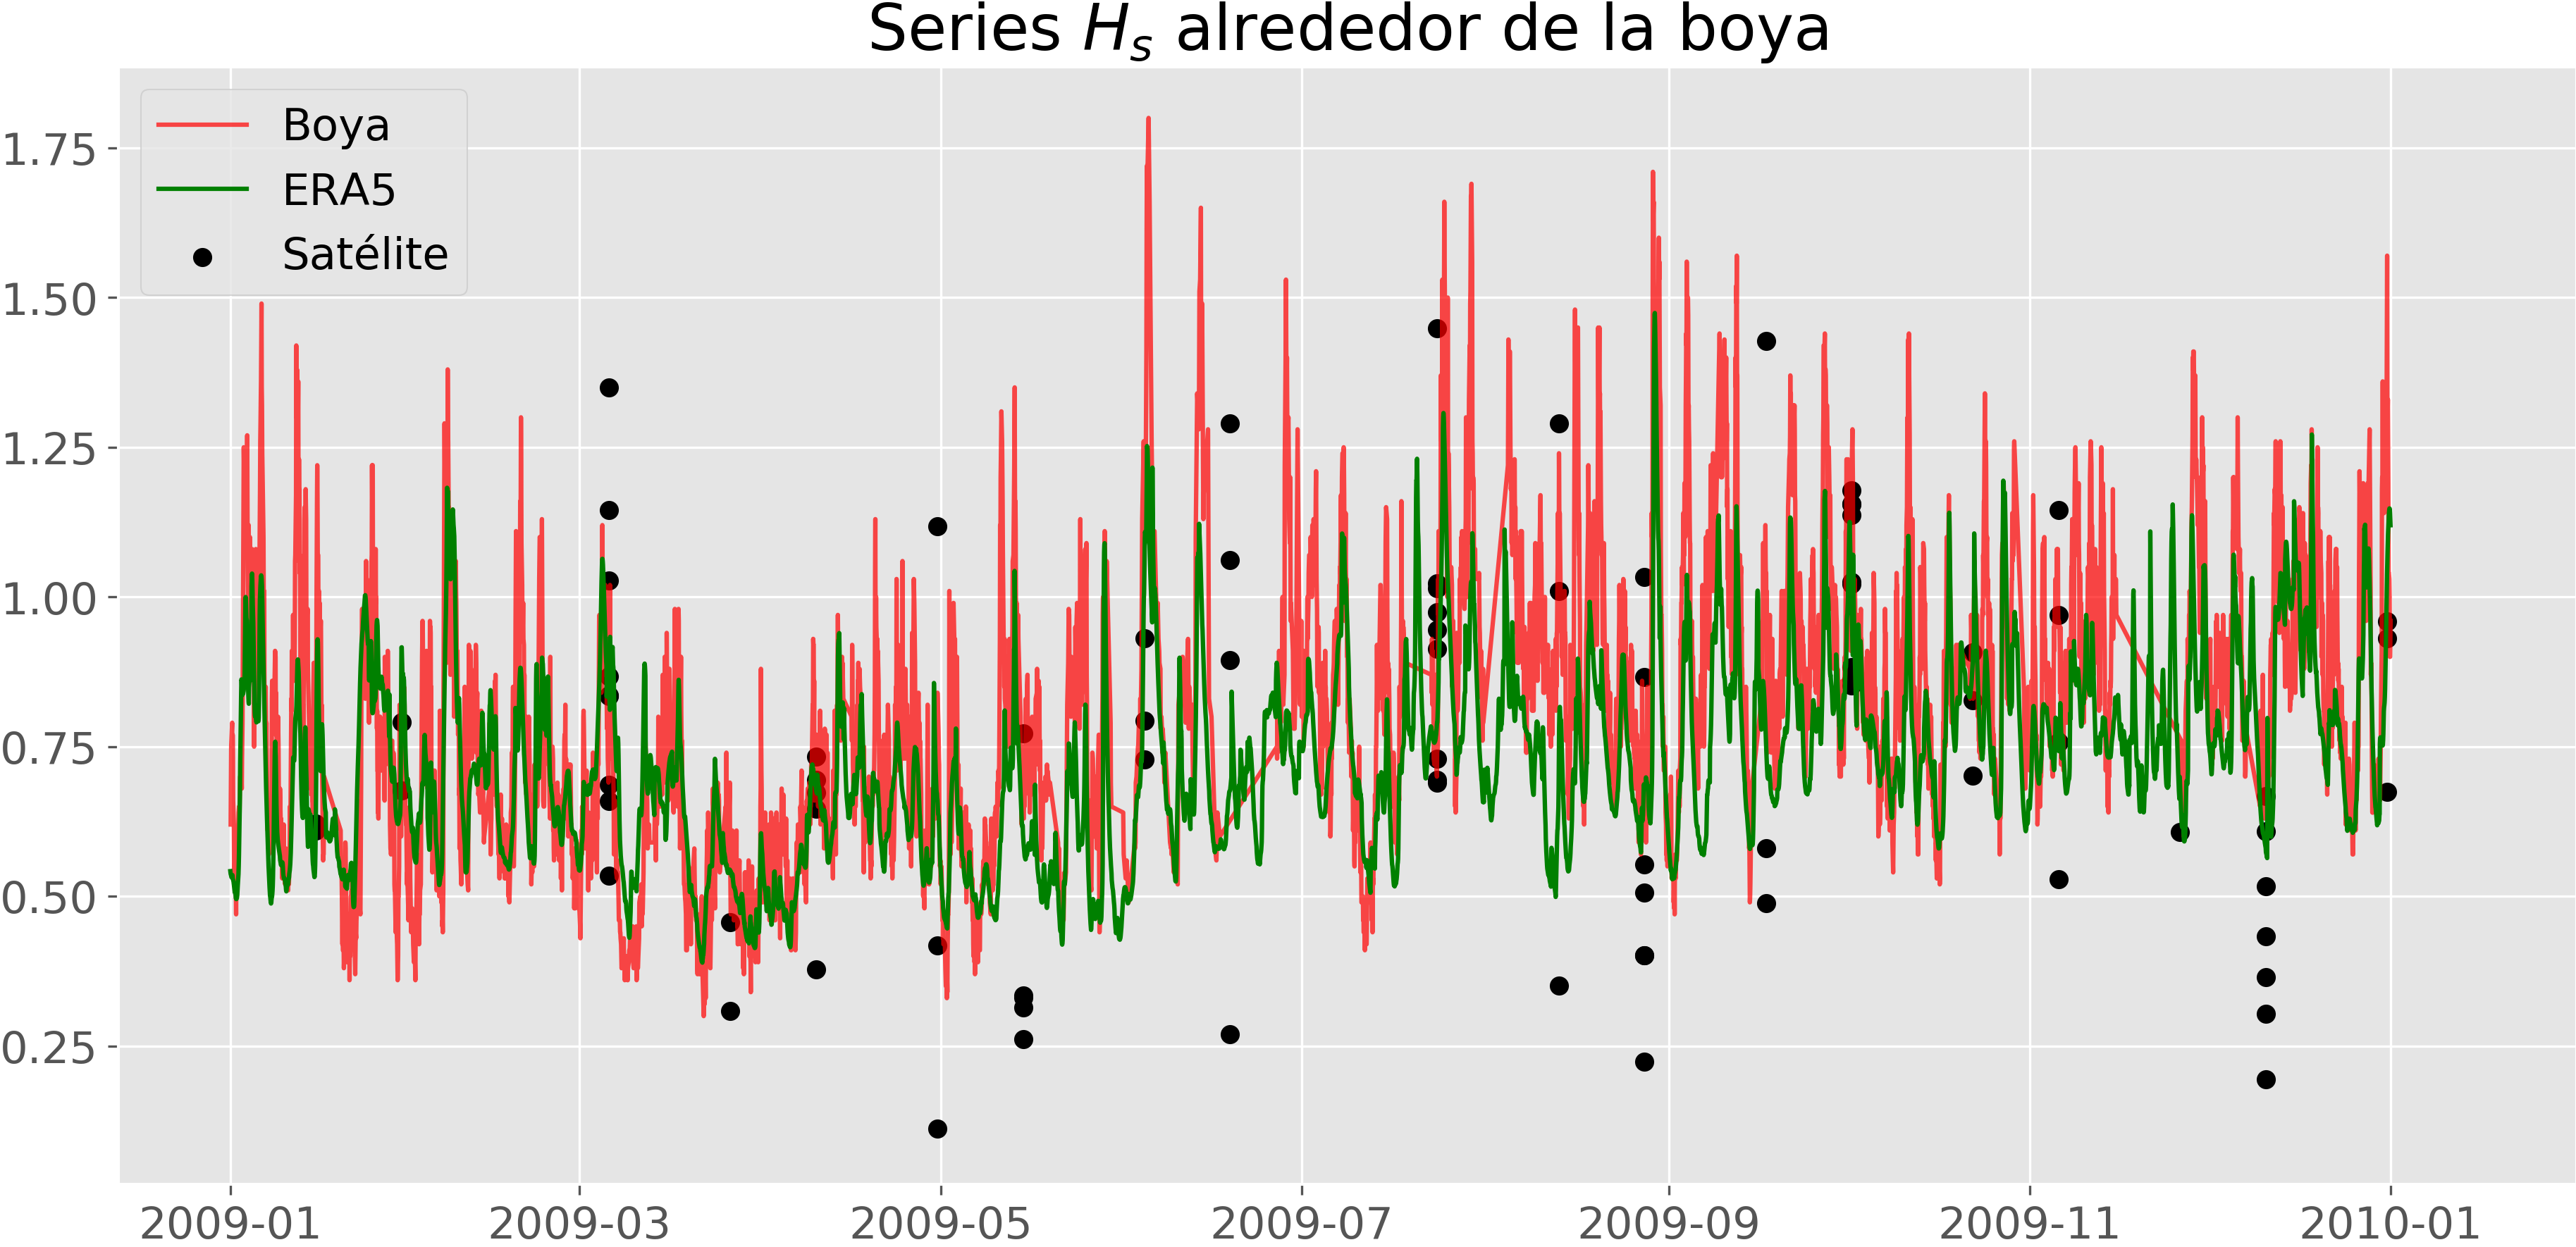
\includegraphics[scale=0.28]{Graficas/Serie1}
    \caption{Series temporales de $H_s$ obtenidas}
    \label{fig:1}
\end{figure}

Para comparar los restantes de una mejor forma, debe igualarse la resolución temporal de las series, esto se realiza mediante una reindexación de la serie de reanálisis, es decir, un ajuste de la resolución presentada por ésta respecto a la resolución presentada por la boya (Fig. \ref{fig:2}). Este procedimiento sólo se puede realizar en este sentido dado que la longitud del registro de reanálisis es mayor.

\begin{figure}
    \centering
    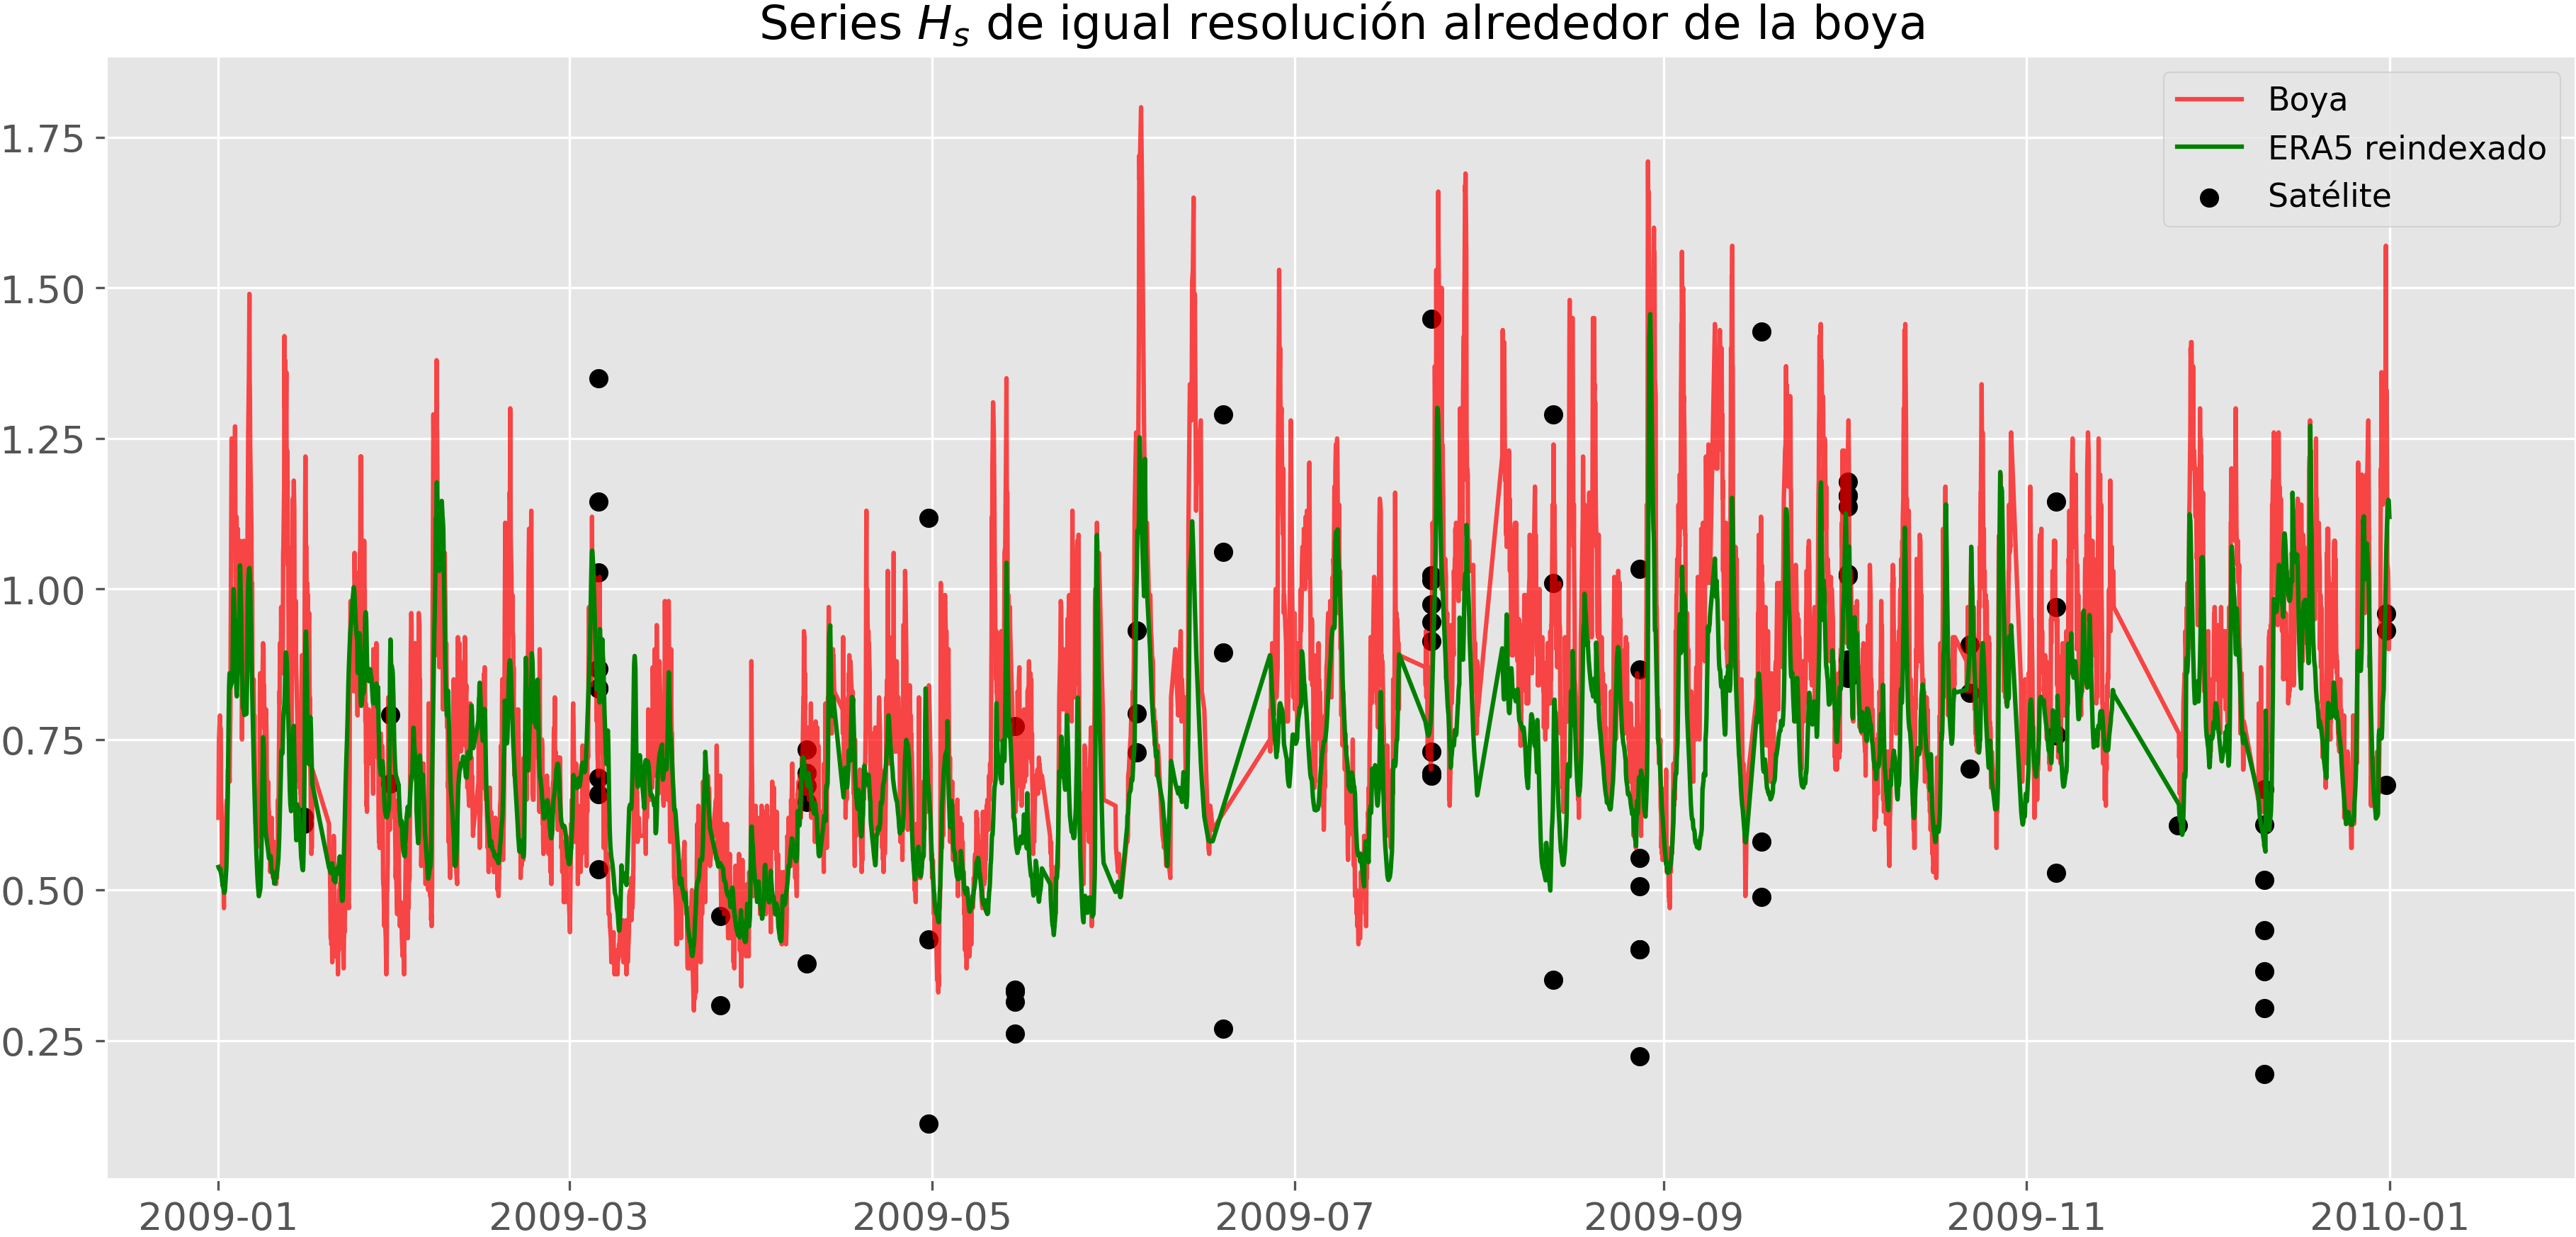
\includegraphics[scale=0.28]{Graficas/Serie2}
    \caption{Series temporales de $H_s$ ajustadas}
    \label{fig:2}
\end{figure}

En la figura \ref{fig:2} con las serie reindexada, el reanálisis logra captura en buena medida los cambios en la magnitud y los valores mínimos de altura de ola significante respecto a la boya, sin embargo, no logra representar los valores máximos. Con el fin de notar esta diferencia, se realiza una comparación de estas series (reanálisis vs boya) en el dominio de la probabilidad a través de un qqplot; este gráfico confronta los cuantiles de una serie respecto a otra, así se conoce sí una serie subestima o sobrestima los valores reales.

\begin{figure}[h]
    \centering
    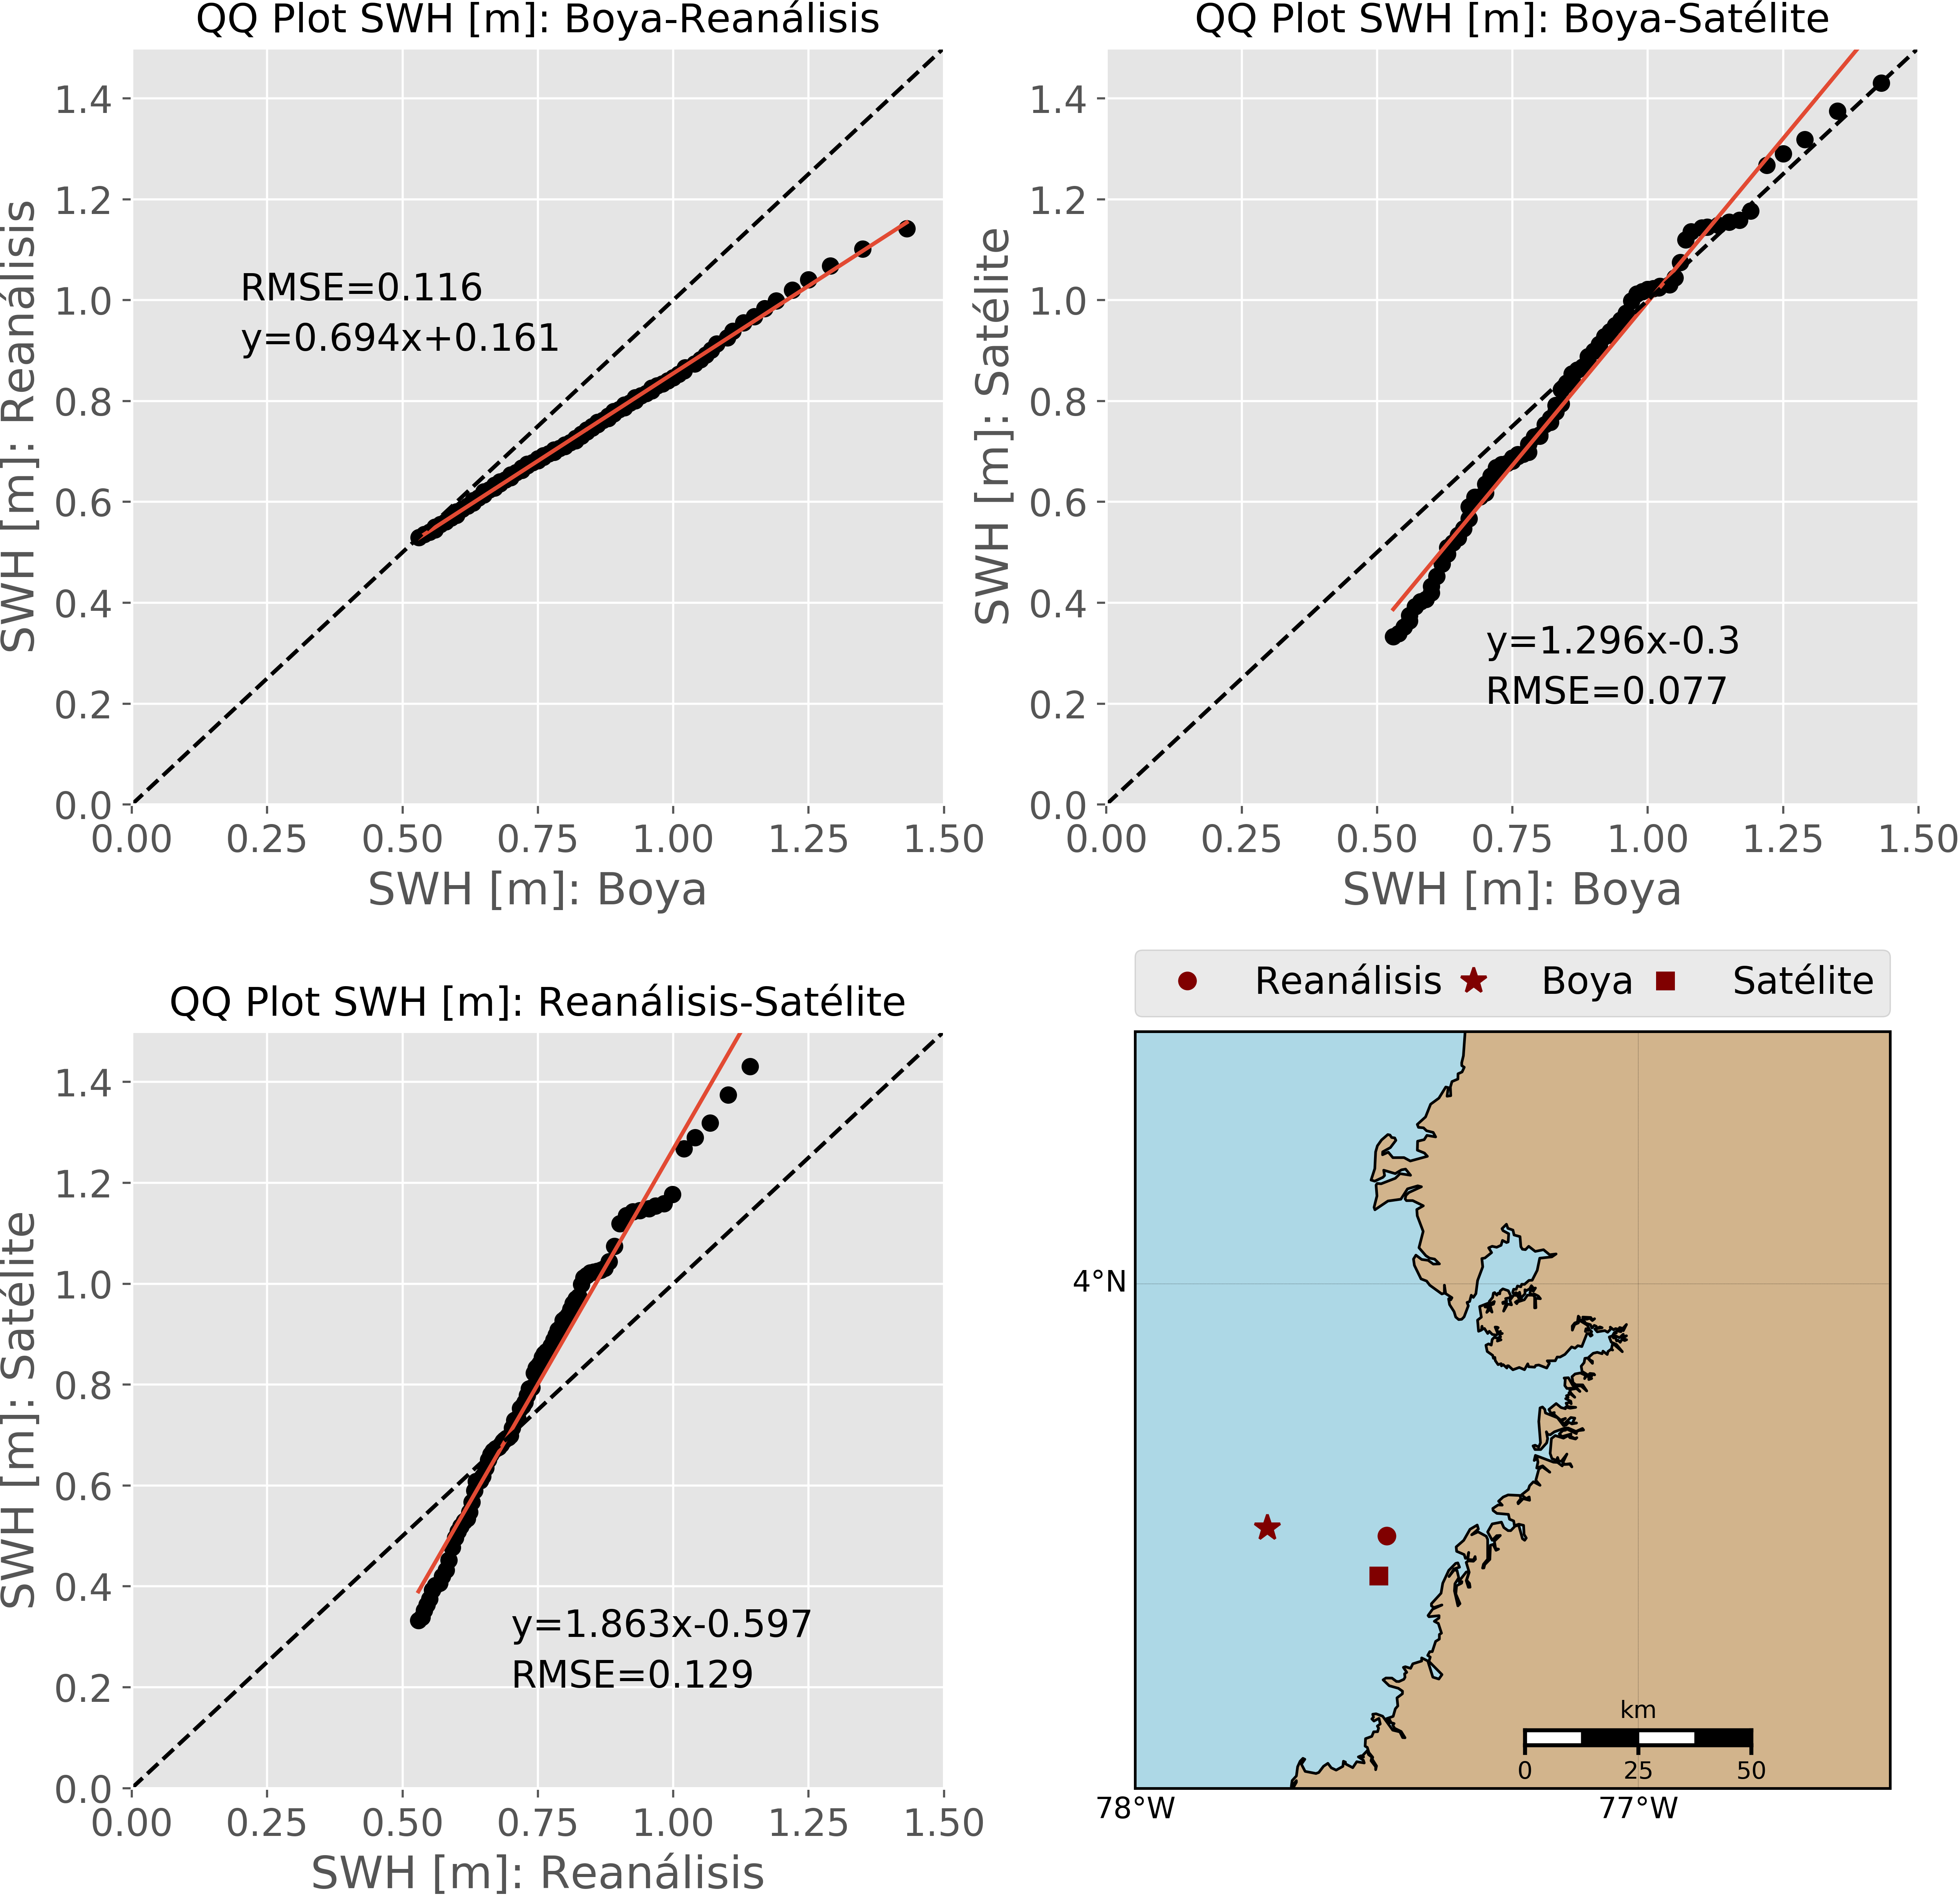
\includegraphics[scale=0.28]{Graficas/QQplots}
    \caption{QQplots para $H_s$}
    \label{fig:3}
\end{figure}

Se ha decidido involucrar los datos satelitáles con el fin de comparar las estimaciones que realiza respecto a las otras fuentes de datos disponibles, puede concluirse a partir de la figura \ref{fig:3} que:

\begin{itemize}
    \item Reanálisis subestima los valores reales de la boya, es decir, entre más grande es el valor de altura de ola, más se aleja el valor de reanálisis por debajo.
    
    \item El satélite, por el contrario, en el primer segmento subestima los valores de la boya, pero después adopta una buena predicción conforme avanzan los valores de altura de ola.

    \item En el primer segmento del gráfico entre el satélite vs el reanálisis, es decir, en los primeros valores de altura de ola significante, el satélite subestima al reanálisis. Posteriormente pasa a sobrestimarlo a medida que aumentan los valores de altura de ola. En este caso se asumen los datos de reanálisis como más veraces y seguros que los satalitales.
\end{itemize}

Reconociendo que los registros de reanálsis no sólo presentan un mejor ajuste frente a los de la boya (\textbf{rmse,pearson}) sino que es la única fuente de datos con registros continuos y en resoluciones temporales buenas y bien definidas, se decide descargar los datos existentes en ERA5 ya no sólo para 2009, sino desde 1973 (primer año de registros) hasta 2018. La descarga de estos datos dada la densidad que reprentan, se realiza con el API request del usuario creado en ERA5. Cada archivo representa un año de datos de período pico, altura de ola significante y dirección del oleaje y está en formato netCDF.

\subsection{Climatología de olas}

Con el fin de caracterizar el régimen medio del oleaje presente en la zona, se analiza la variación anual y estacional a lo largo de la longitud del registro (xx años)

\subsubsection{Variación anual}

La figura \ref{fig:4 variacion anual} muestra la varación anual de la altura de ola significante ($H_s$), período pico ($T_p$) y dirección media (Dir). El valor medio anual de altura de ola es y  el valor máximo presentado es m, para el período pico el valor medio anual es y el valor máximo fue .. s. Es notorio que los valores máximos se presentaron en el año 1985, año en el que se presentó un fenómeno ENSO (El Niño South Oscilation) muy fuerte (\textbf{CITAR}). Otros valores máximos de altura y período también parecen estar ligados a dicho fenómeno macroclimático (años .....). Esta especificación anterior, también permite reafirmar que la altura de ola y el período pico son eventos dependientes,dado que variaciones importantes de uno repercuten sobre el otro, como si de hecho, fuera un sistema acoplado.

La dirección del oleaje presenta variaciones de hasta... La tendencia de la altura de ola promedio anual es m/año y del período pico promedio anual es s/año

\begin{figure}[h]
    \centering
    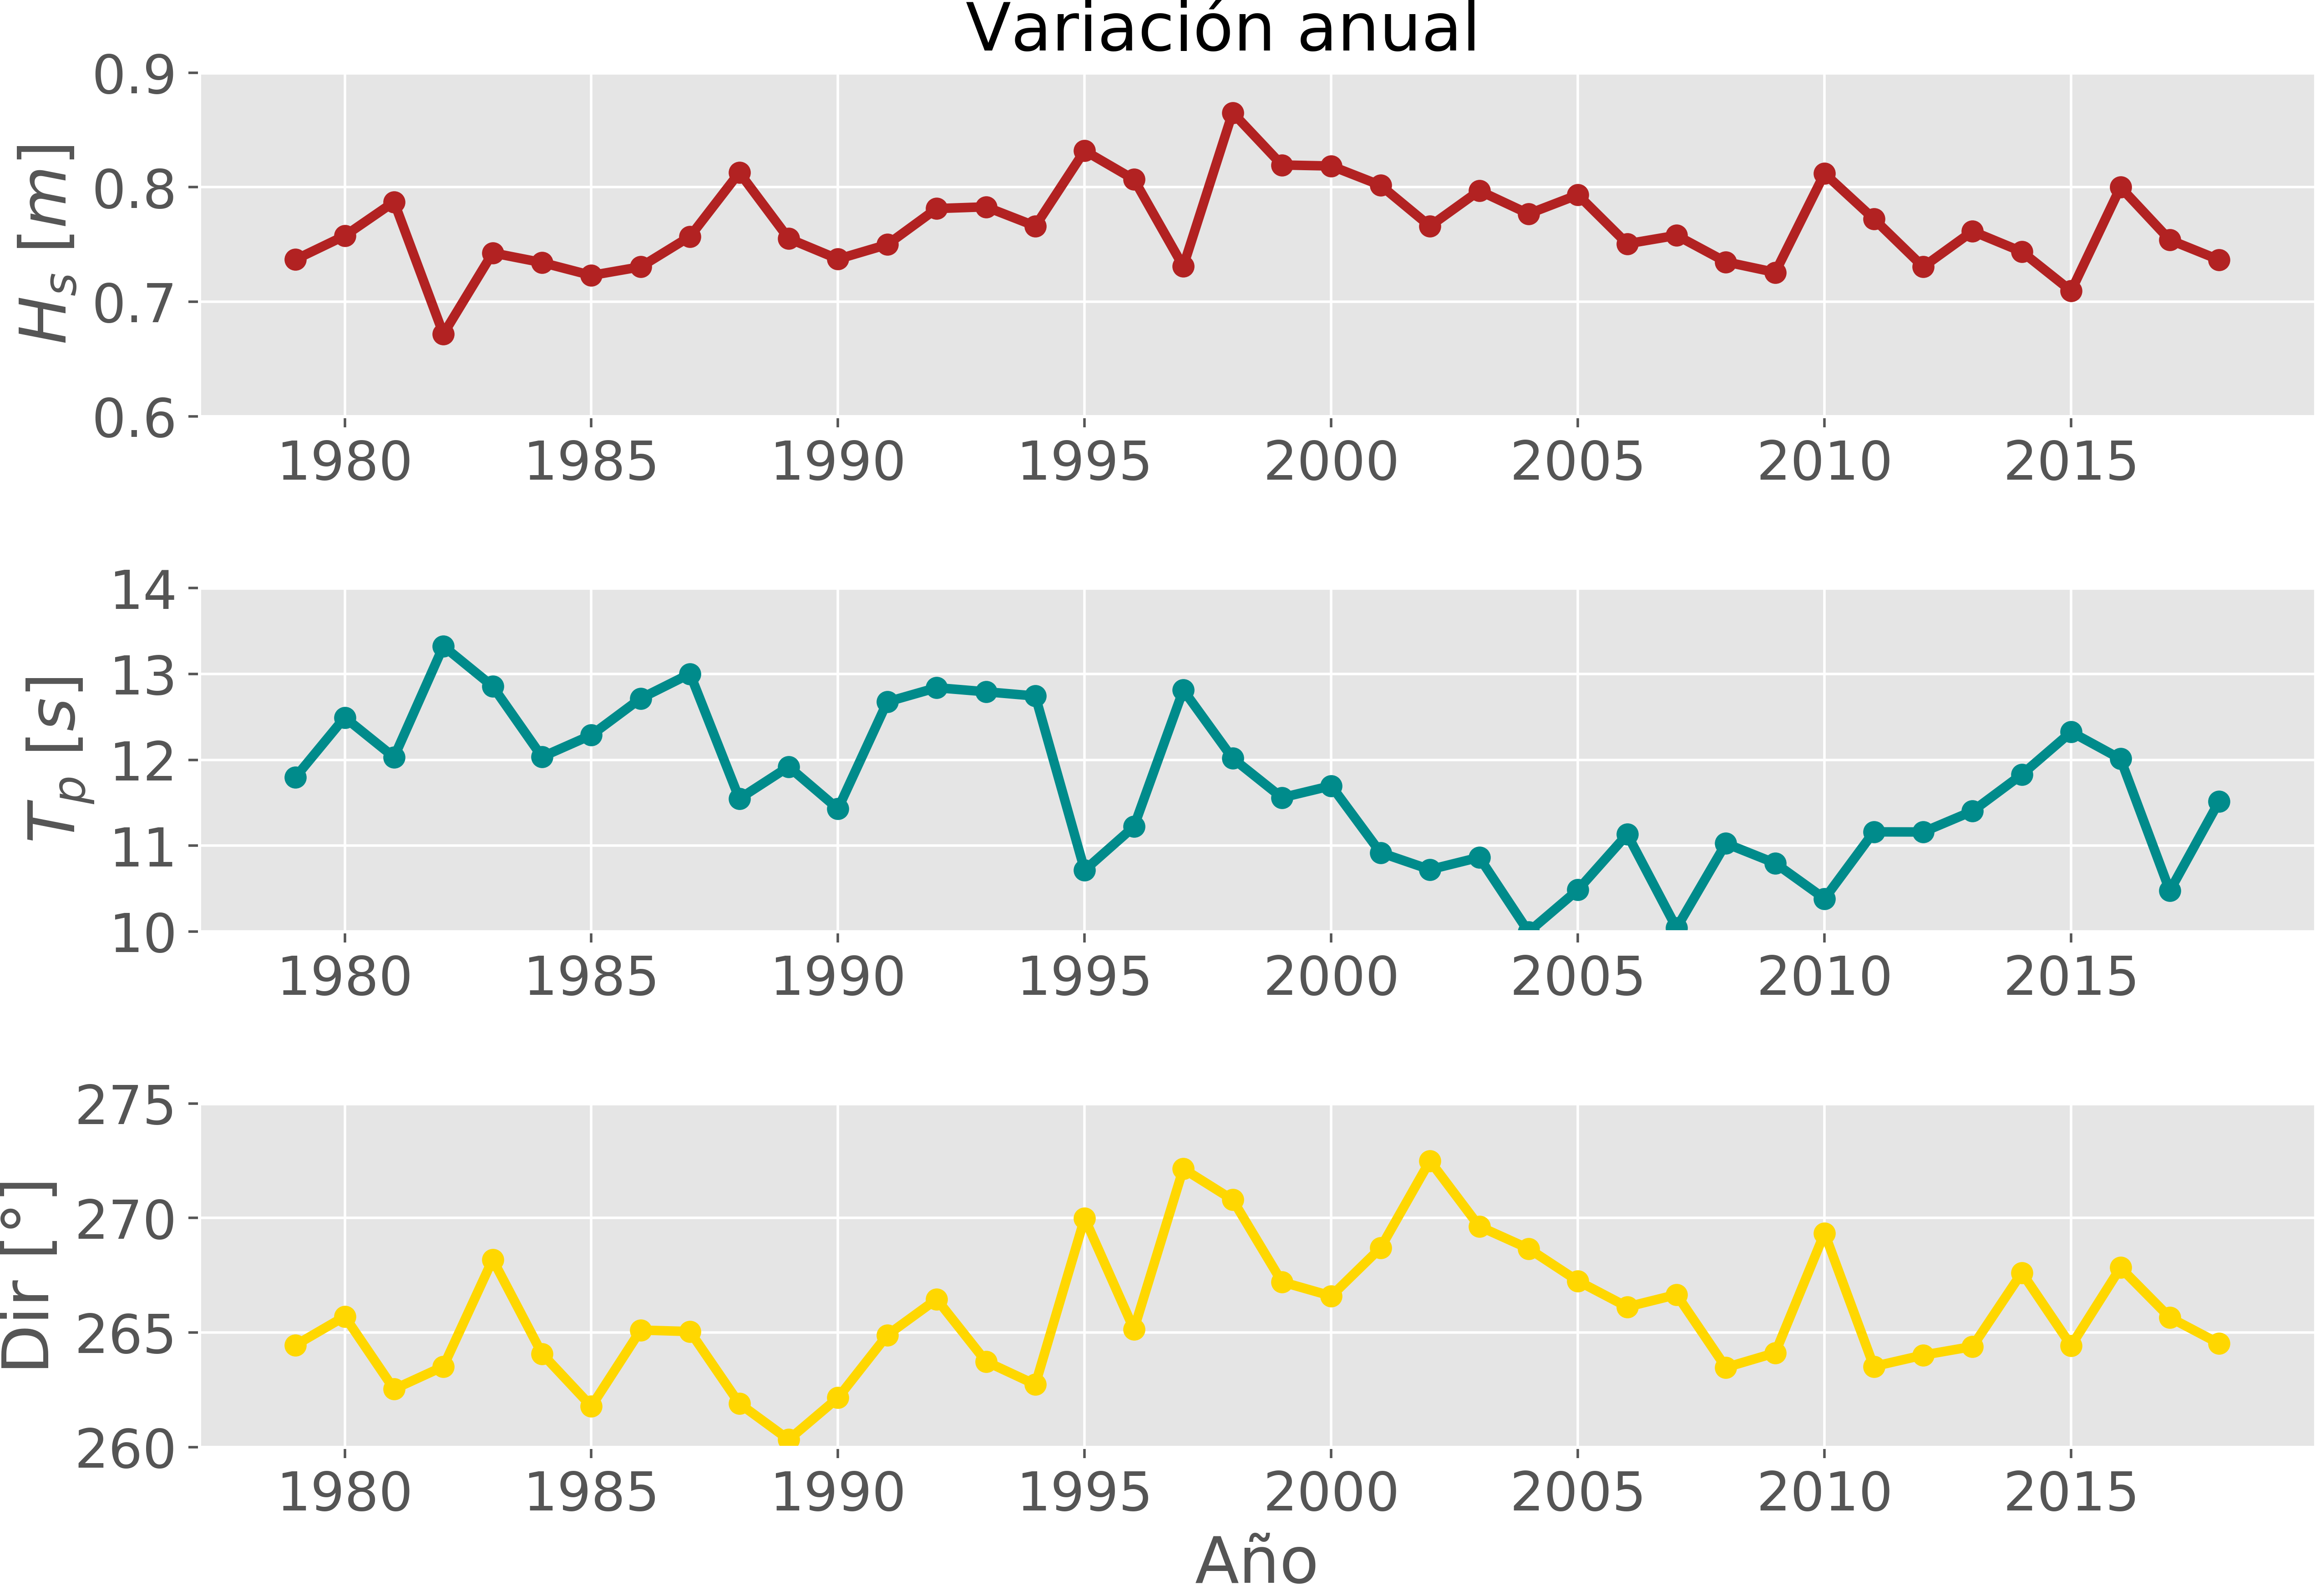
\includegraphics[scale=0.28]{Graficas/Variacion_interanual}
    \caption{variación anual del oleaje}
    \label{fig:4 variacion anual}
\end{figure}

\subsubsection{Variación estacional}

La temporada seca y húmeda en Colombia, está marcada por el paso de la zona de convergencia intertropical (ZCIT), en la primera parte del año (Enero-Junio) se presenta la temporada seca, esto debido a que la ZCIT se encuentra en la posición más al sur de su recorrido, esto permite el paso de los vientos alisios del noreste, estos vientos como forzadores generan el mayor oleaje desde esa zona. Cuando la ZCIT se traslada hacia el norte, permite la entrada de los vientos alisios del sureste, según la figura \ref{fig:5 ciclo anual} se espera un oleaje más energético desde esta dirección, aunque deberá corroborarse con una rosa de oleaje.

\begin{figure}[h]
    \centering
    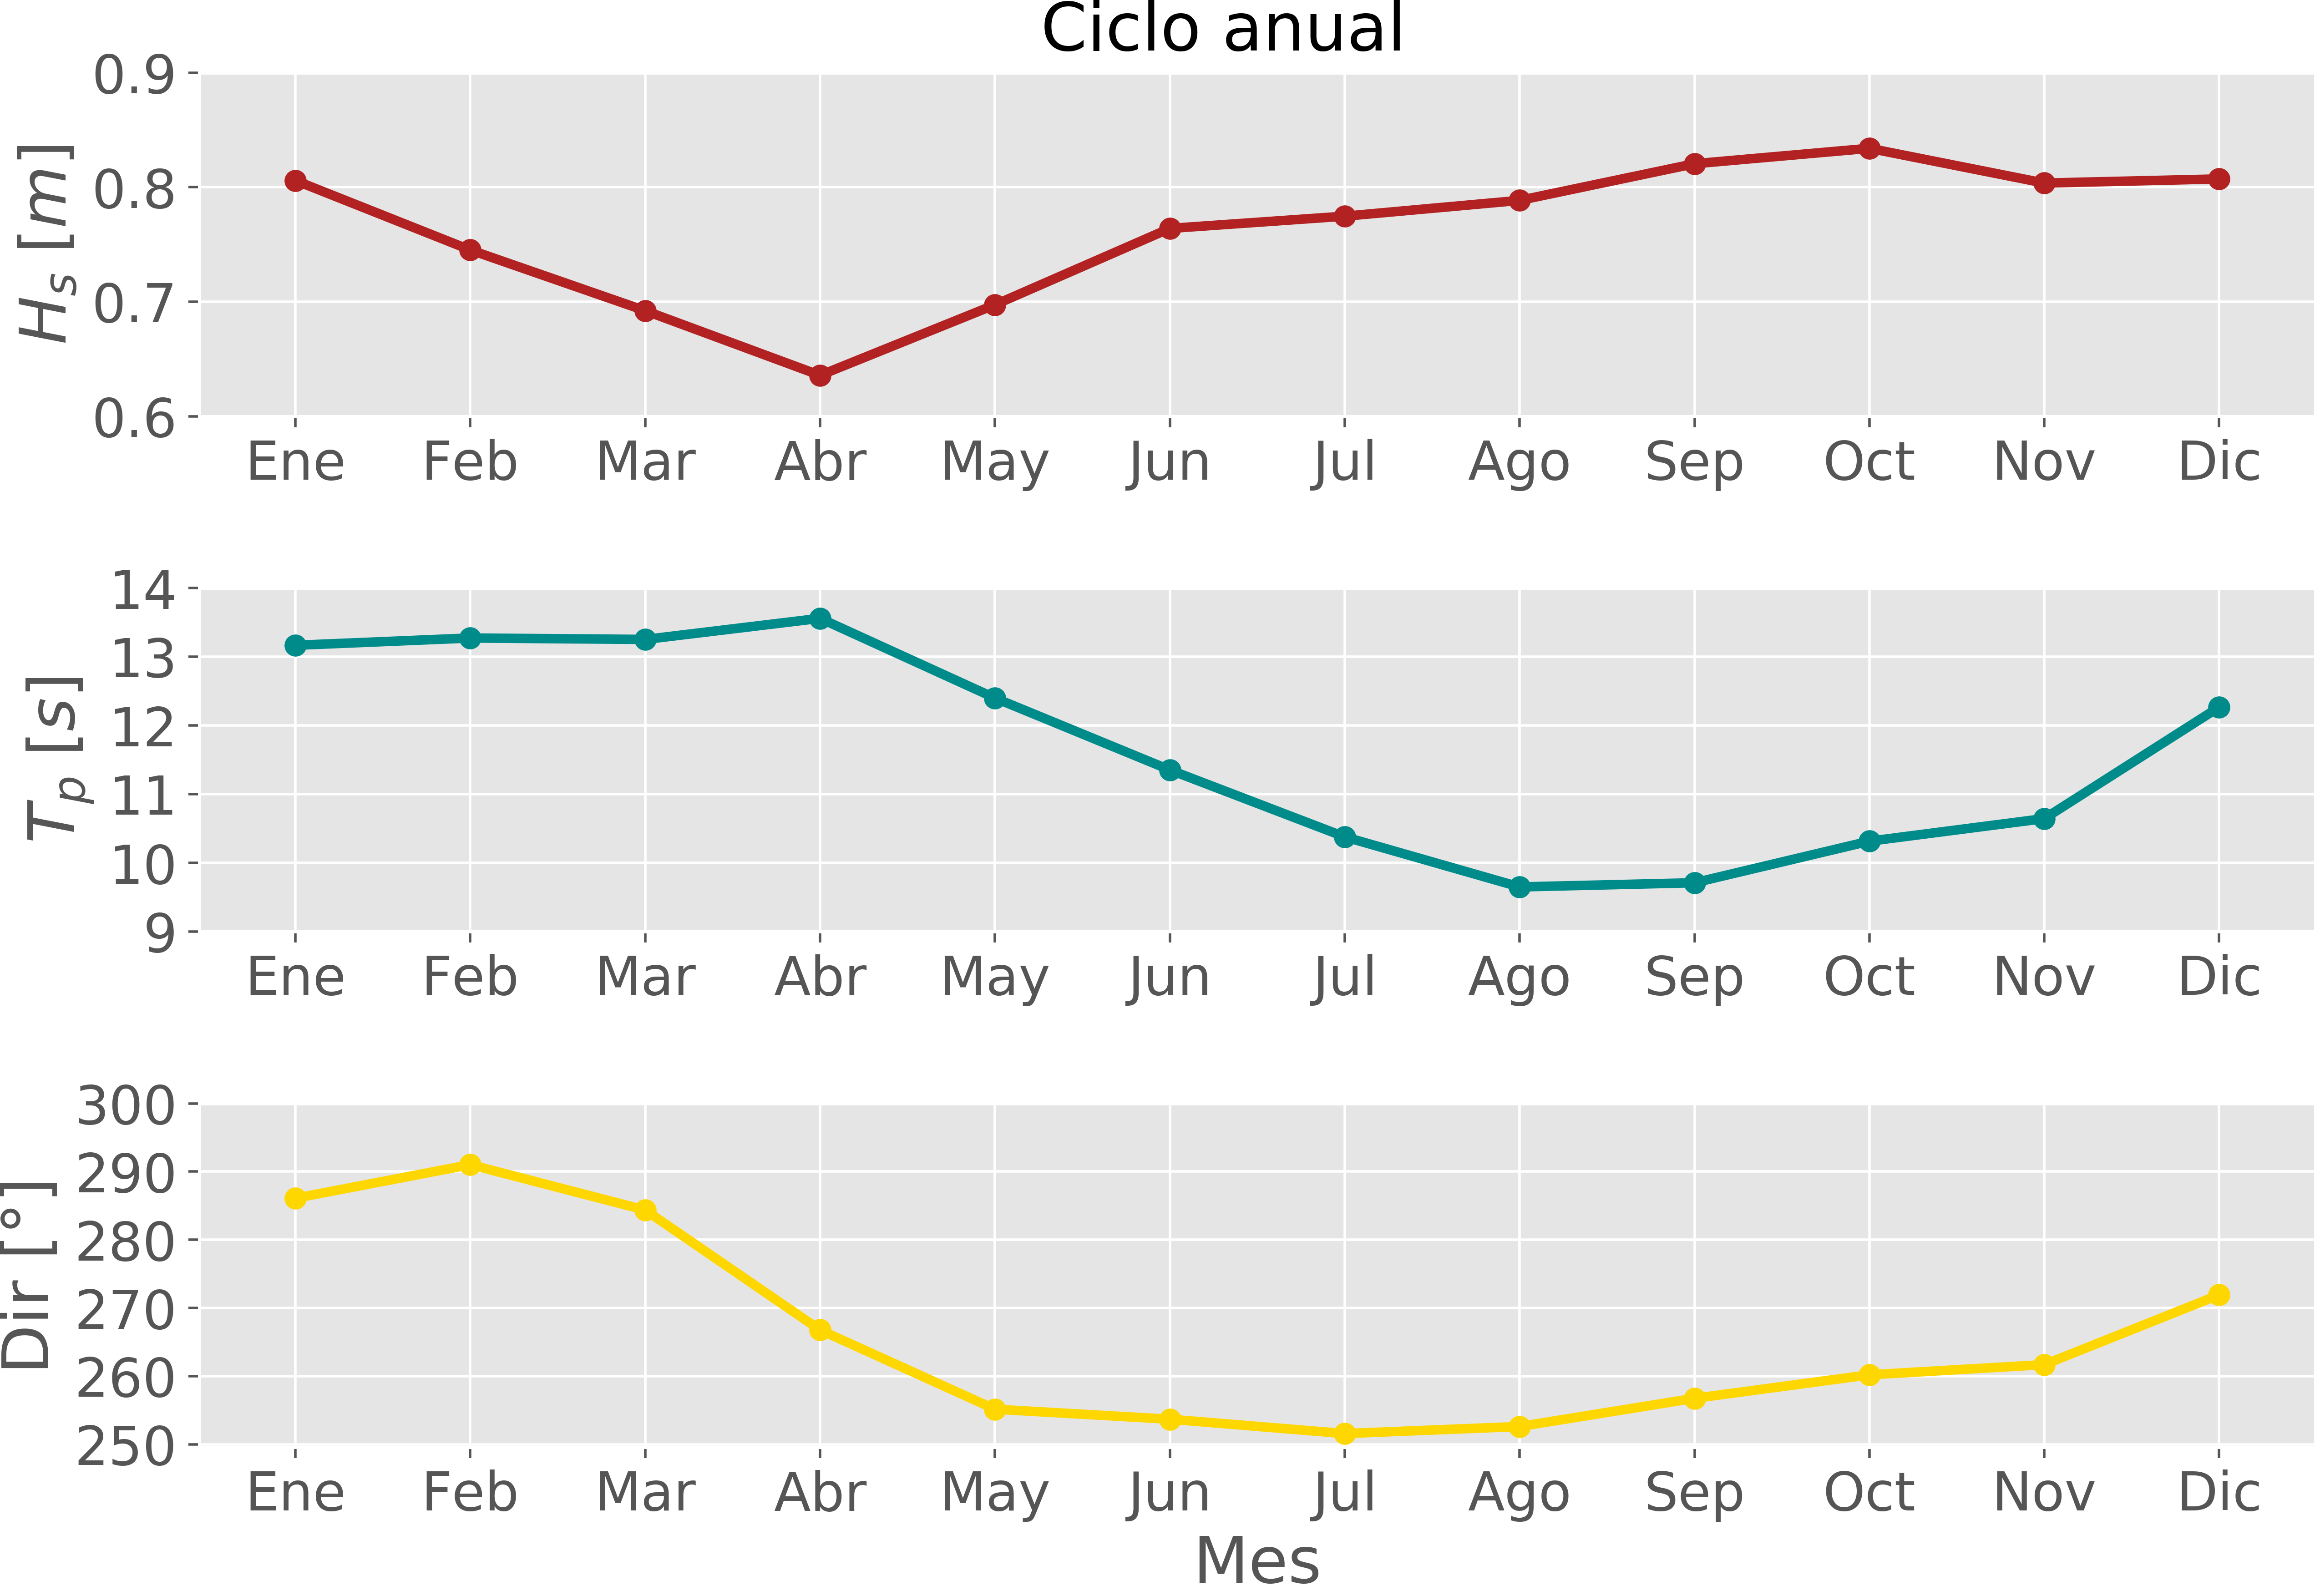
\includegraphics[scale=0.28]{Graficas/Ciclo_anual}
    \caption{Ciclo anual del oleaje}
    \label{fig:5 ciclo anual}
\end{figure}

La dirección del oleaje presenta una variación del norte al sur entre los meses.. la variación mensual es de 

\subsection{Análisis de marea}
La series del nivel der mar descargadas, representan la marea presente en la zona. Cómo es bien sabido, la márea está compuesta por una parte astrónomica (deterministica) y otra parte aleatoria (estocástica), se requiere entonces realizar, en primera medida, un análisis armónico de dicha serie para determinar la marea astronómica, con dicho análisis se determinan las las componentes solares y lunares más inciden sobre la zona de estudio y con estas, se determinan las amplitudes de dicha marea.

La herramienta utilizada para el análisis armónico es el script t\_tide.py, basado en la rutina t\_tide desarrollada inicialmente para Matlab por \textbf{CITAR}. Este script exige dos condiciones iniciales que deben cumplir las series de nivel del mar para poder determinar a cabalidad las componentes de dicha marea

\begin{itemize}
    \item Menor a 18.6 años: Esta condición existe debido a que el cabeceo de la luna, es decir, su cambio orbital, ocurre en este intervalo de tiempo. Por lo tanto, cada 18.6 años la marea astronómica es igual y determinándola para dicha franja de tiempo se puede determinar para muchos años más.
    \item Continuidad de la serie: Cuando la serie de nivel del mar tiene muchos huecos, así sean llenados con valores \textit{NaN}, las componentes de la marea se alejan de su valor verdadero.
\end{itemize}

\subsubsection{Proceso de llenado}
Para poder obtener una serie homogénea debe reconstruirse 

De la tabla .. puede notarse que las componentes M2,S2,N2,K1 y K2 son las que más aportan a la amplitud, en especial M2, por lo que la conclusión es que la marea en la zona es de tipo semidiurna.


\section{Resultados}

\subsection{Eventos medios}
Para determinar los eventos medios, primero debe reconocerse que existe un oleaje que incide desde diferentes direcciones, por lo tanto debe graficarse una rosa de oleaje que represente dichas condiciones.

\begin{figure}[h]
    \centering
    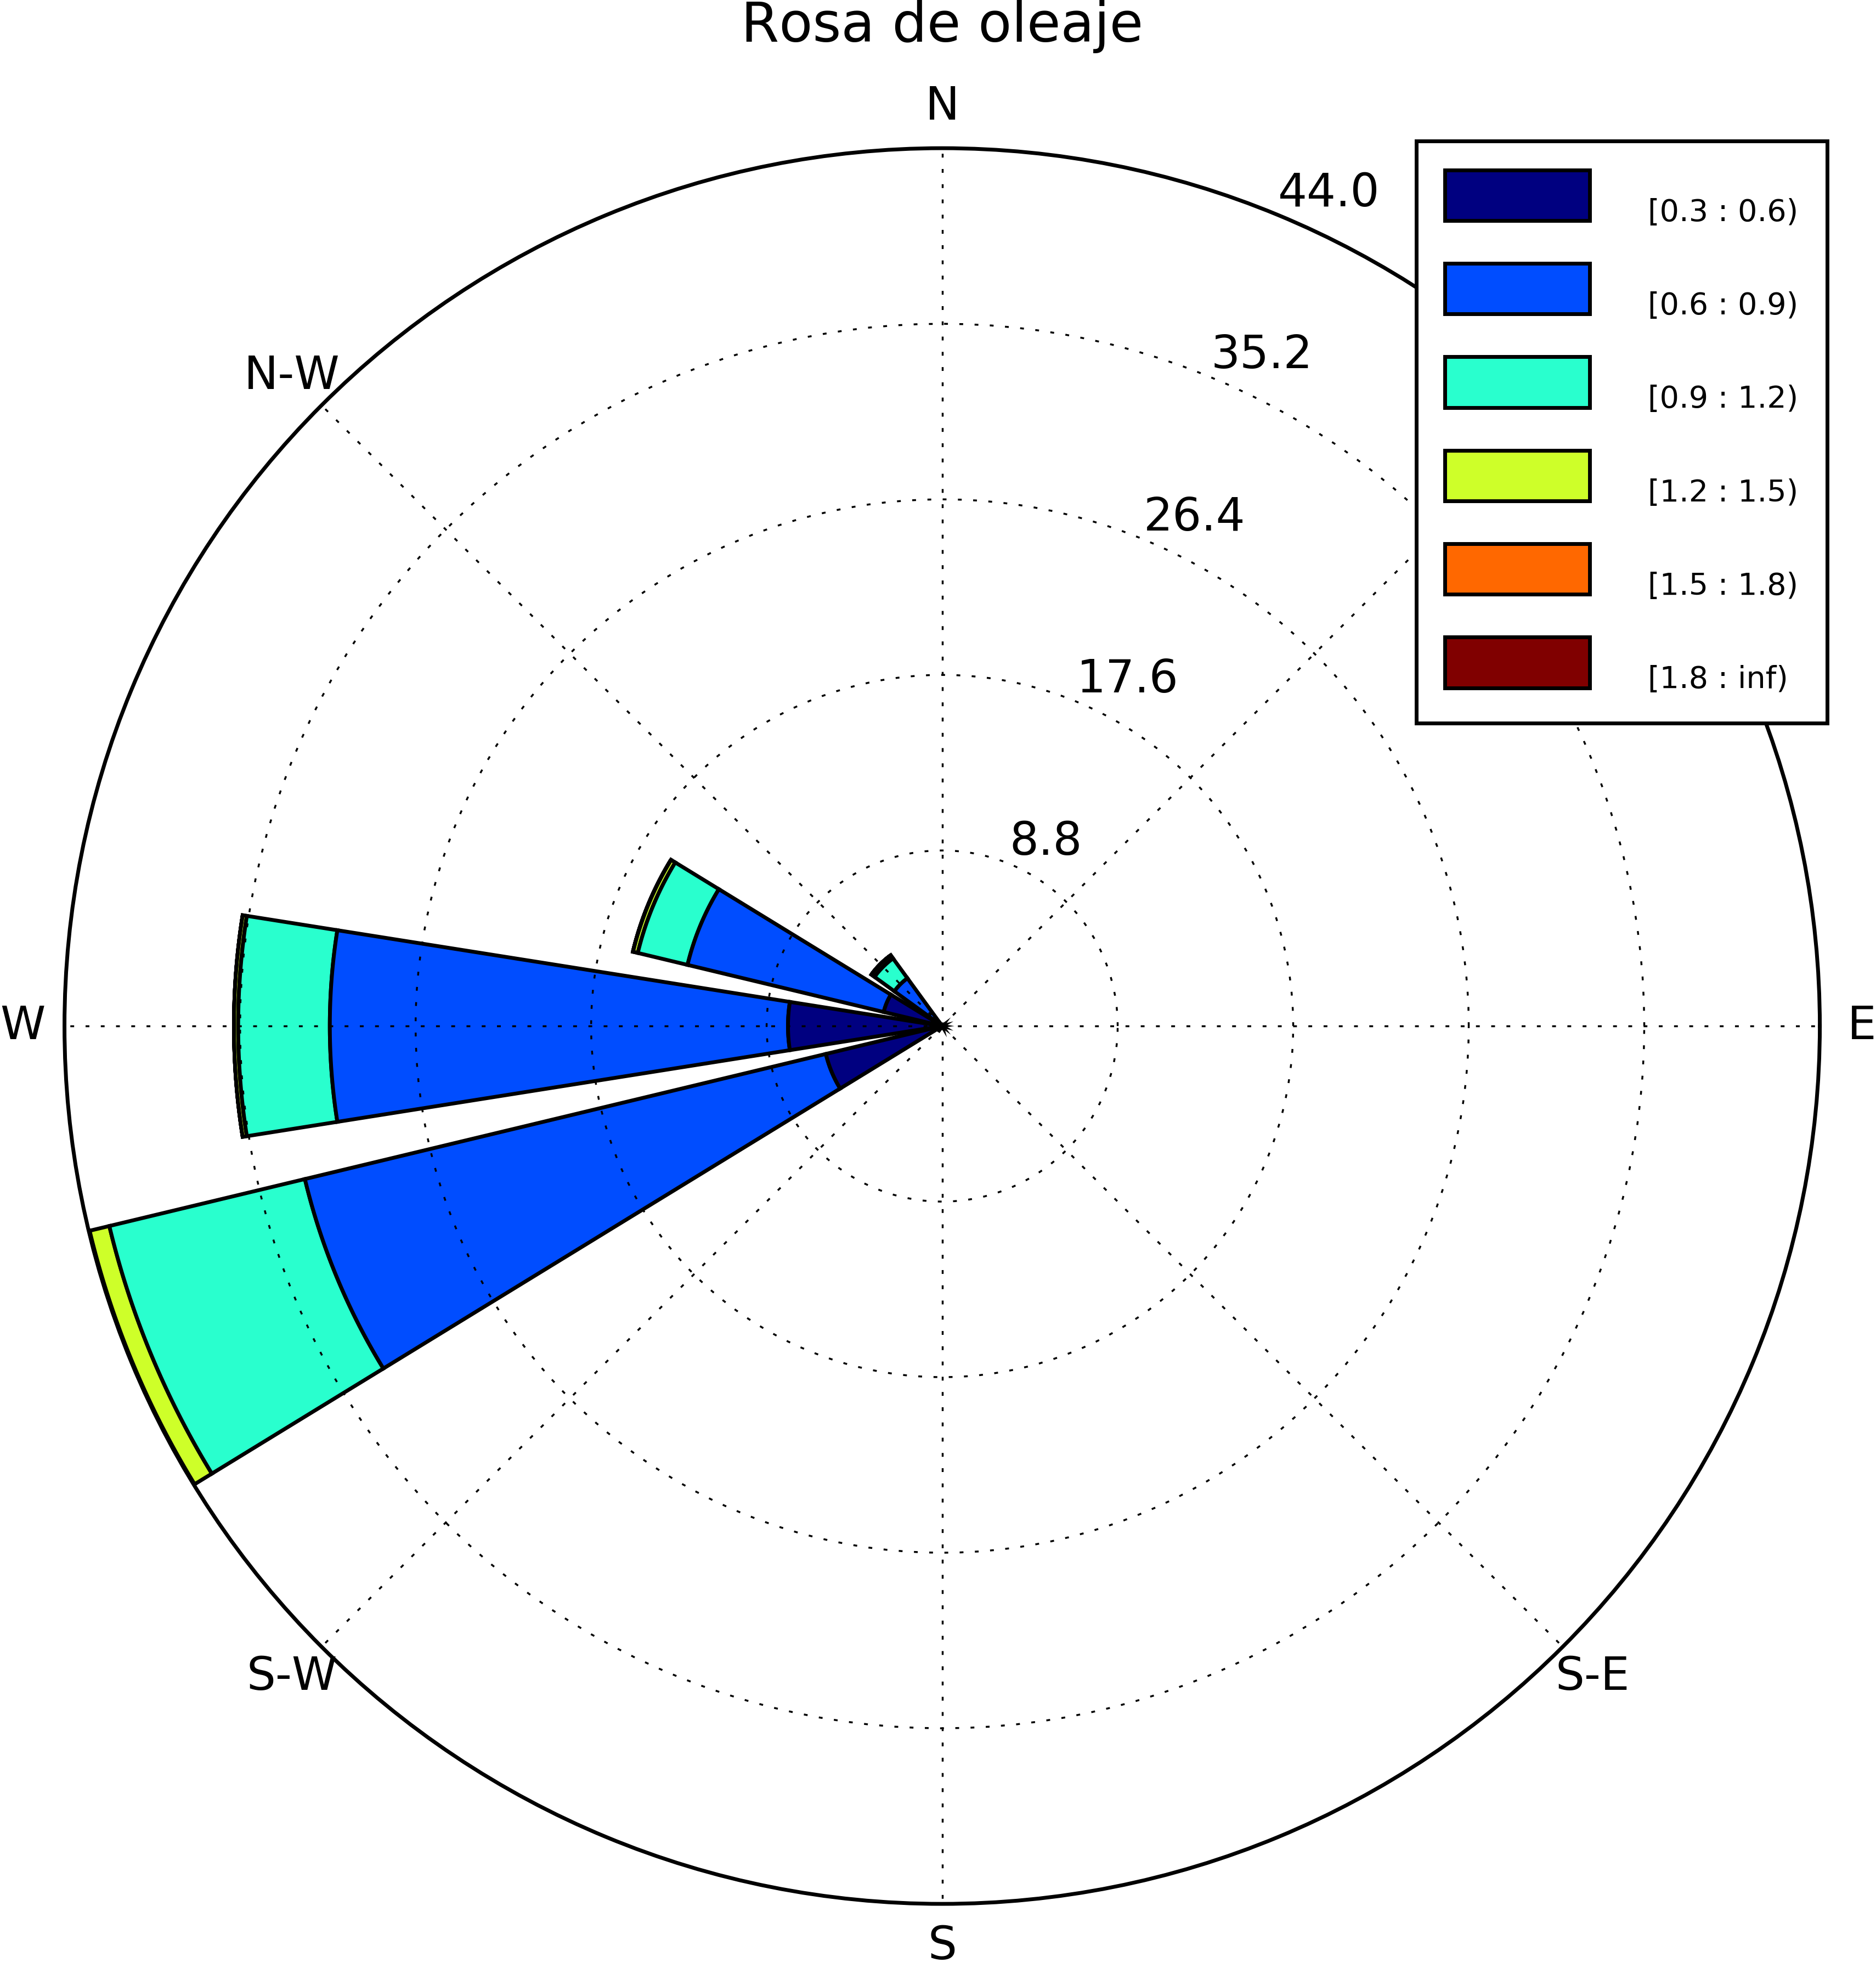
\includegraphics[scale=0.35]{Graficas/rosa_oleaje}
    \caption{Rosa de oleaje}
    \label{fig:6 Rosa de oleaje}
\end{figure}

La rosa de oleaje muestra las direcciones principales del oleaje, la frecuencia que tienen cada una de ellas y las respectivas alturas de olas significantes . El campo de dirección se compone de 16 zonas de 12.5$^\circ$ cada una, esto  discretiza el dominio direccional, útil en el uso posterior de modelos de propagación.

Tal como lo relata ...  y cómo puede notarse en la figura \ref{fig:5 ciclo anual}, el oleaje comienza al principio del año en una dirección sur oeste y al final del año va avanzando hacia el norte, dejando sus principales registros en lass direcciones W y WSW con cerca del 70\% de los datos (Fig.\ref{fig:7 Prob direccional}). Otras direcciones importantes son, aunque con probabilidades más bajas.

\begin{figure}[h]
    \centering
    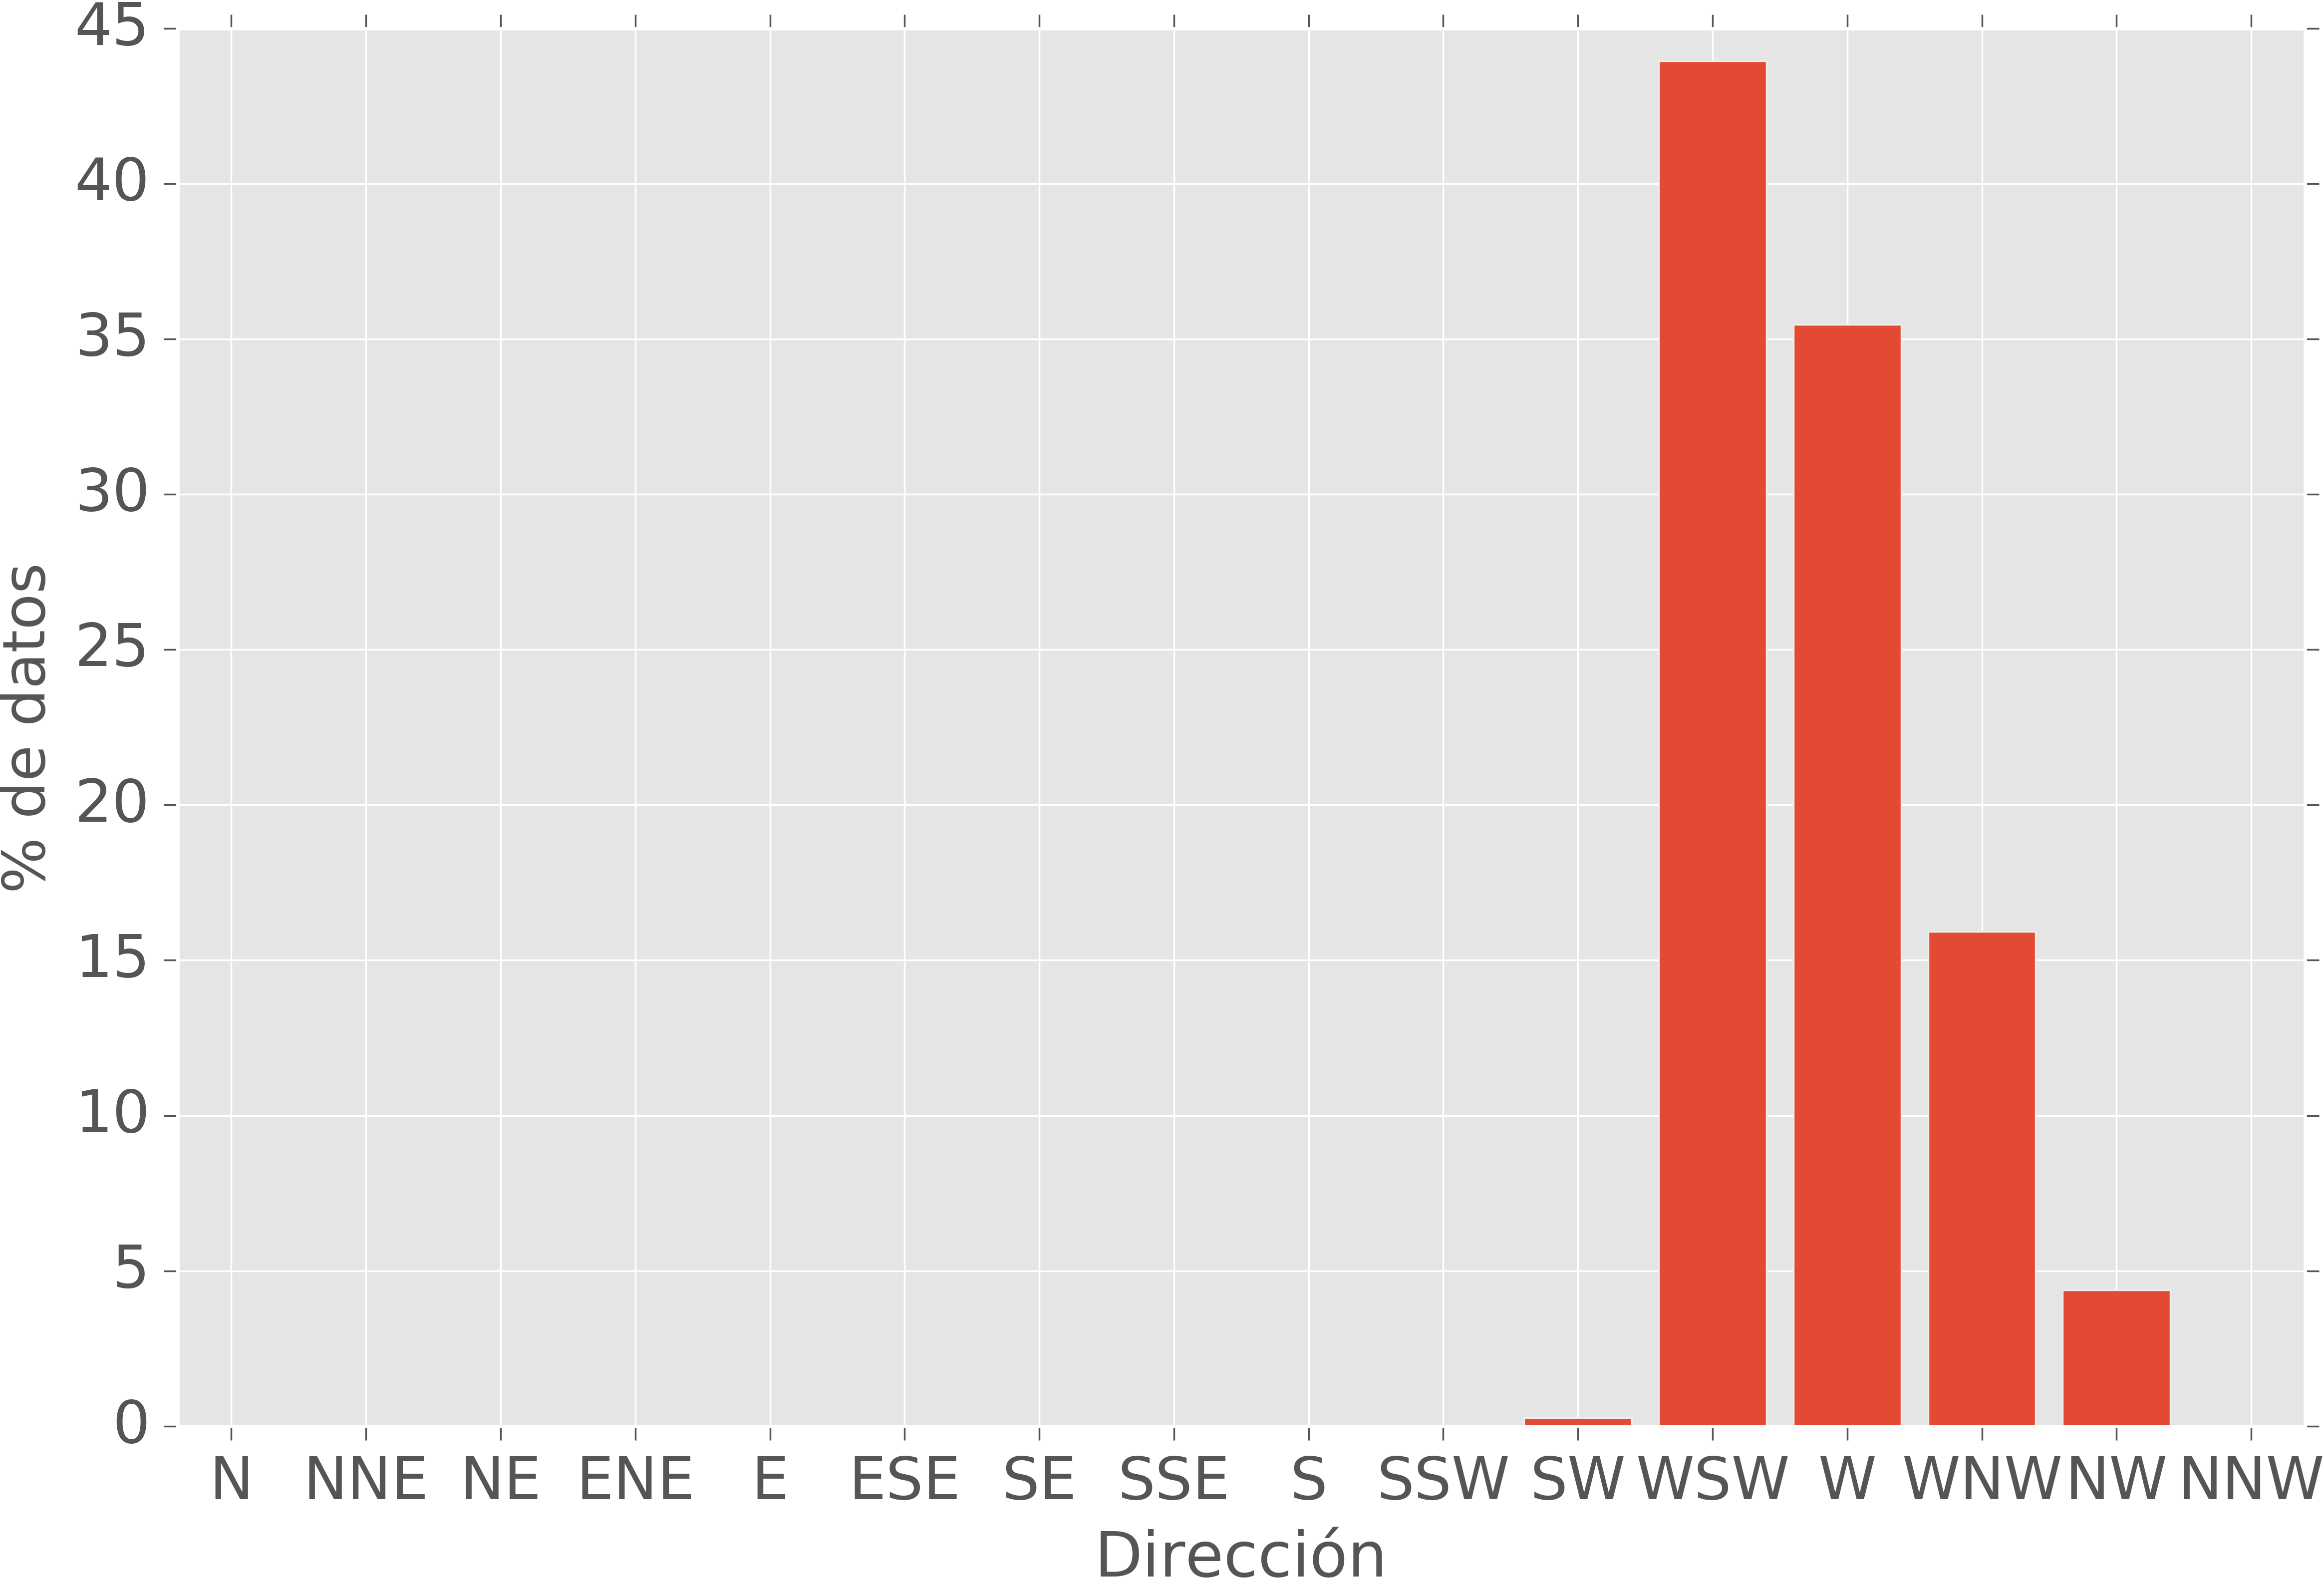
\includegraphics[scale=0.35]{Graficas/histograma_direccional}
    \caption{Probabilidad direccional}
    \label{fig:7 Prob direccional}
\end{figure}

Posteriormente, se filtra el registro temporal a través de éstas direcciones y a partir de los histogramas bivariados entre $H_s$ y $T_p$ para cada dirección, se determina en cada región ($x,y$), el número de duplas ($H_s,T_p$) que quedaron contenidas. El objetivo de estos histogramas es la determinación de la probabilidad conjunta, la cual se define como la probabilidad de ocurrencia de una pareja de valores de Hs y Tp.

\begin{figure}[h]
    \centering
    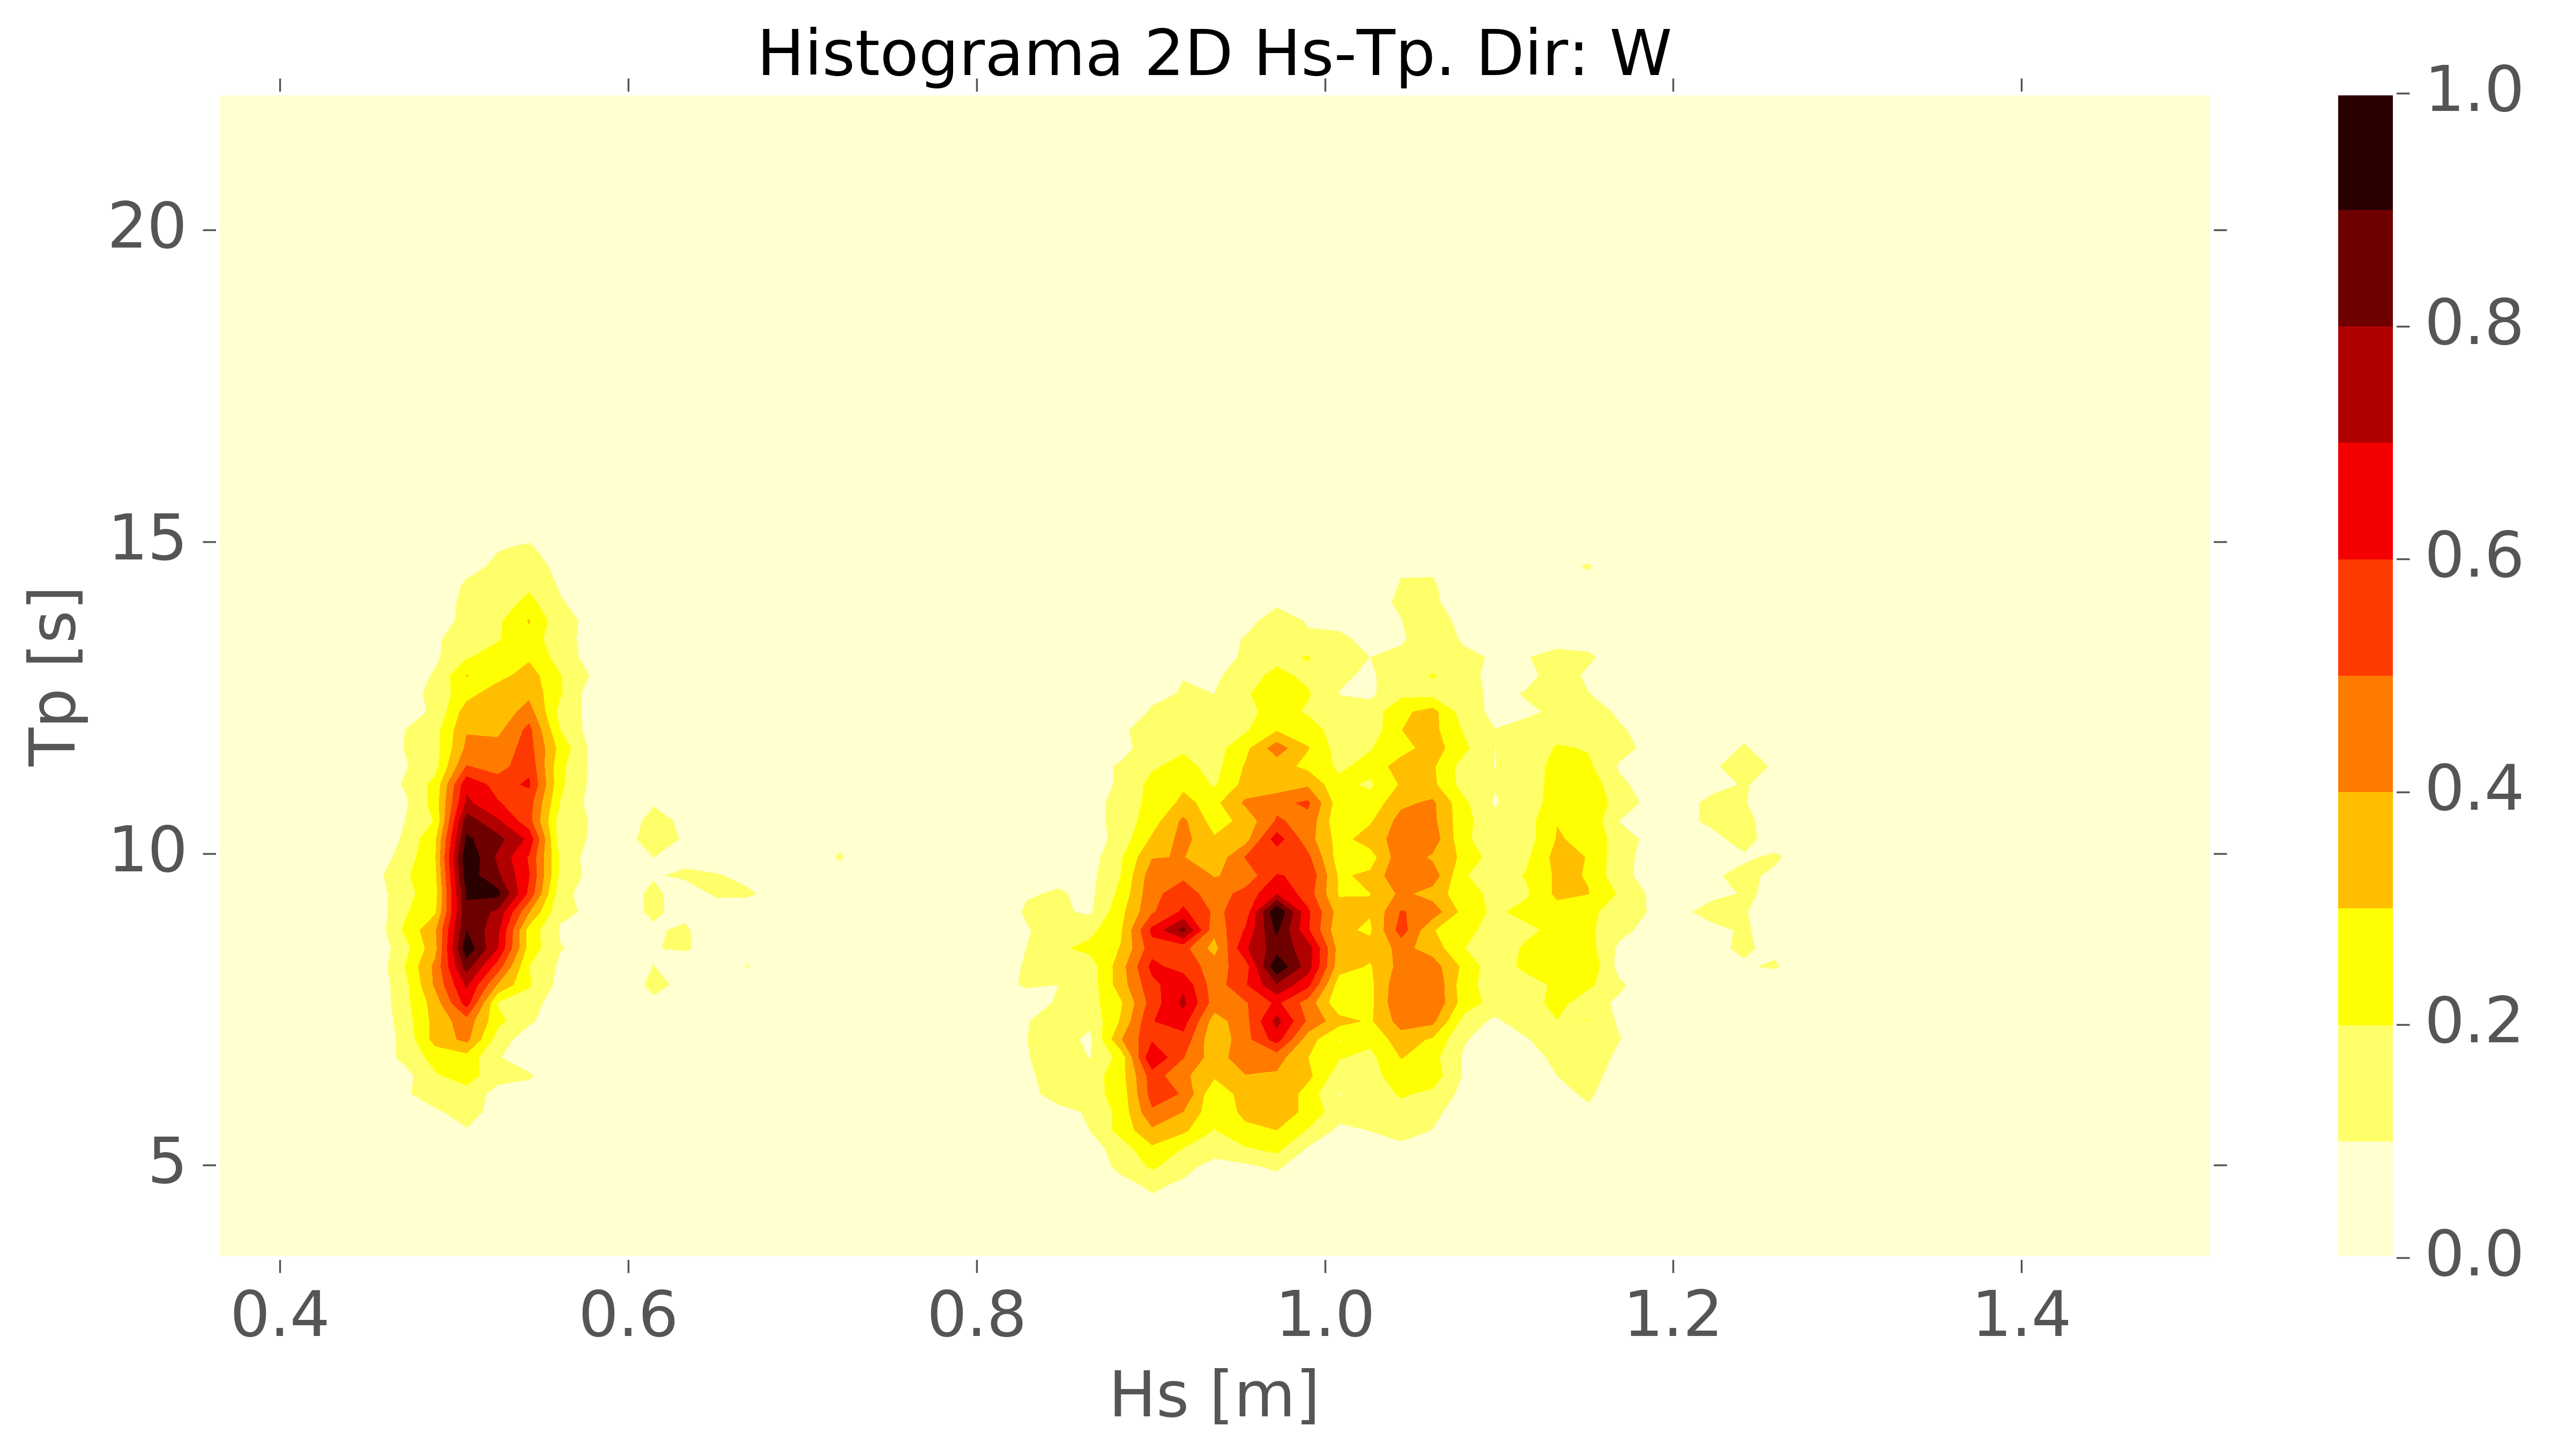
\includegraphics[scale=0.28]{Graficas/Histograma2d_W}
    \caption{Probabilidad conjunta $H_s-T_p$}
    \label{fig:8 Prob conjunta}
\end{figure}


Los gráficos de probabilidad conjunta finalmente determinan los casos más representativos del oleaje para cada una de las direcciones (Hs-Tp-Dir), elegidos en un uso posterior, como parámetros de entrada para los modelos de propaganda de oleaje.


\subsection{Nivel del mar}

\section{Conclusiones}


%%%%%%%%%%%%%%%%%%%%%%%%%%%%%%%%%%%%%%%%%%%%%%%%%%%%%%%%%%%%%%%%%%%%%%%%%%%%%%%%%%%%%%%%
%% ATENCION AUTORES: ESTA SECCION ES OBLIGATORIA
%%%%%%%%%%%%%%%%%%%%%%%%%%%%%%%%%%%%%%%%%%%%%%%%%%%%%%%%%%%%%%%%%%%%%%%%%%%%%%%%%%%%%%%%

\section*{Agradecimientos}


\label{}

%% The Appendices part is started with the command \appendix;
%% appendix sections are then done as normal sections
%% \appendix

%% \section{}
%% \label{}

%% References
%%
%% Following citation commands can be used in the body text:
%% Usage of \cite is as follows:
%%   \cite{key}         ==>>  [#]
%%   \cite[chap. 2]{key} ==>> [#, chap. 2]
%%


%% References with BibTeX database:

\bibliographystyle{elsarticle-harv}


\appendix
\section{Primer Apandice}    % Capa Apandice debe tener un tatulo corto.
Este texto esta repetido. Si utiliza Word, use o bien Microsoft Editor de Ecuaciones o
MathType  para las ecuaciones de su artaculo (Insertar | Objeto |
Crear Nuevo | Microsoft Editor de Ecuaciones o Ecuacian MathType).
No debe seleccionar la opcian ``Flotar'' sobre el texto. Por
supuesto, LaTeX gestiona las ecuaciones a travas de macros
pre-programadas.

Listo está bien

\end{document}

%%
%% End of file `ejemplo latex RIAI.tex'.